\chapter{MODELAGEM E SIMULAÇÃO}\label{cap:processo}

\section{MODELO FÍSICO}

A planta é uma haste rígida que gira em torno de um eixo fixo. O empuxo $F$ é a entrada e o ângulo $\theta$ em relação à horizontal (positivo quando o motor sobe) é a variável regulada. A soma dos torques sobre o pivô fornece a segunda lei de Newton para a rotação, na mesma forma usada em plataformas 1DOF descritas na literatura \cite{mane2019,cuero2020,uyar2024}:
\begin{equation}
 J\ddot\theta=l_mF-g\,S_m\cos\theta-b\dot\theta+\tau_d
 \label{eq:modelo}
\end{equation}
em que $J$ é o momento de inércia em torno do pivô, $l_m$ o braço do motor, $S_m$ o momento estático das massas em relação ao pivô (positivo do lado do motor), $b$ o atrito viscoso e $\tau_d$ um torque externo. O empuxo responde ao comando $u$ (PWM) com dinâmica de primeira ordem de constante $\tau_m$:
\begin{equation}
 \tau_m\dot F=F_{\max}\,u-F
\end{equation}
Na horizontal o termo $\cos\theta$ tem derivada nula, de modo que, em torno de $\theta=0$, a planta se comporta como um integrador duplo com atraso de primeira ordem. Isso explica por que um controle apenas proporcional oscila e por que a ação derivativa é indispensável.

\section{IDENTIFICAÇÃO NA BANCADA}

Não há dados confiáveis de massa e empuxo do kit. Em vez de estimá-los, a planta foi identificada com o próprio firmware, a partir dos registros de ângulo e saída gravados na RAM em 6 de outubro de 2026. O modelo reduzido da Equação~\ref{eq:modelo}, escrito direto em graus e em porcentagem de PWM, foi ajustado a dois registros feitos com ganhos diferentes:
\begin{table}[htbp]
\centering\caption{Parâmetros da planta identificados na bancada.}\label{tab:parametros}
\begin{tabularx}{\textwidth}{Xrl}
\hline\textbf{Parâmetro} & \textbf{Valor} & \textbf{Origem}\\\hline
Ganho do atuador & $\approx 300^\circ/\mathrm{s}^2$ por 1\% de PWM & ajuste ao registro\\
PWM para pairar & $\approx 20{,}2\%$ (16 a 23\% nos registros anteriores) & partida de 02/11/2026\\
Atraso do empuxo $\tau_m$ & $\approx 58$ ms & ajuste ao registro\\
Atraso puro (filtro do sensor e amostragem) & $\approx 9$ ms & ajuste ao registro\\
Repouso (haste caída) & $\approx -38^\circ$ & leitura do sensor\\
Limite de saída & 32\% & projeto (Seção~\ref{sec:potencia})\\\hline
\end{tabularx}
\fonte{Elaborado pelos autores (2026), com \texttt{firmware/tools/arm\_margins.py} e \texttt{firmware/tools/arm\_tune.py}.}
\end{table}
A frequência de oscilação prevista pelo modelo para os ganhos usados na segunda rodada foi 18,4~rad/s; a medida na bancada foi 18~rad/s, o que sustenta a identificação. O modelo é de pequenos sinais em torno do ponto de pairar e não representa zona morta nem a não linearidade da curva PWM--empuxo. Massa, inércia e braços não foram medidos; a pesagem das peças permanece como trabalho futuro.

\section{CONTROLE E MARGENS DE ESTABILIDADE}

Com a planta identificada, a margem de fase foi calculada pela resposta em frequência da malha (PID com derivada filtrada, integrador duplo, atraso de empuxo e atraso puro). Com os ganhos iniciais ($K_p=1{,}0$, $K_i=0{,}5$, $K_d=0{,}15$), a haste ficou em ciclo-limite entre $-10{,}8^\circ$ e $+5{,}4^\circ$, com a saída batendo nos limites. Com $0{,}30/0{,}15/0{,}09$, a margem de fase era de só $3{,}6^\circ$ e a haste oscilou $\pm3{,}7^\circ$. Os ganhos de projeto, $K_p=0{,}06$, $K_i=0{,}05$ e $K_d=0{,}04$, com filtro da derivada de 5~ms, foram escolhidos para ter cerca de $43^\circ$ de margem de fase nominal e pelo menos $33^\circ$ com o ganho do atuador entre 120 e $380^\circ/\mathrm{s}^2$ por 1\% e o atraso entre 45 e 75~ms. Depois, o refino na bancada subiu $K_i$ para 0,08 (Capítulo~\ref{cap:refino}). A lição é que, com atraso de empuxo de dezenas de milissegundos, ganho alto produz oscilação, e não precisão.

\section{SIMULAÇÃO}

O simulador (\texttt{report/simulation/sim\_1dof.py}, Python com NumPy e Matplotlib) integra o modelo identificado com passo de 5~ms e reproduz o PID do firmware linha a linha: derivada na medida, filtro da derivada, limites de 10\% a 32\%, rampa de saída de 300\%/s e integrador iniciado em 16\% \footnote{Uma versão anterior do trabalho usava um simulador em Drake com parâmetros estimados; ela foi substituída por este modelo, que usa a planta identificada. Os resultados antigos não são reutilizados.}. Esse modelo também existe em C (\texttt{firmware/tests/sim\_control.c}), que compila o \texttt{control.c}, o \texttt{pid.c} e o \texttt{angle\_filter.c} do próprio firmware, de modo que a lógica embarcada é testada no computador.

Usando o PWM de pairar medido na bancada (20,2\%), a simulação leva a haste do repouso, a $-38^\circ$, até a faixa de $\pm2^\circ$ em torno do alvo em cerca de 5,7~s, com sobressinal de cerca de $0{,}3^\circ$ (Figura~\ref{fig:partida}). Na bancada, a mesma partida levou 6,6~s (Capítulo~\ref{cap:resultados}). A subida lenta decorre dos ganhos baixos: o integrador, iniciado em 16\%, é quem sustenta a haste.
\begin{figure}[htbp]
\centering\caption{Partida simulada a partir do repouso, com os ganhos de projeto.}\label{fig:partida}
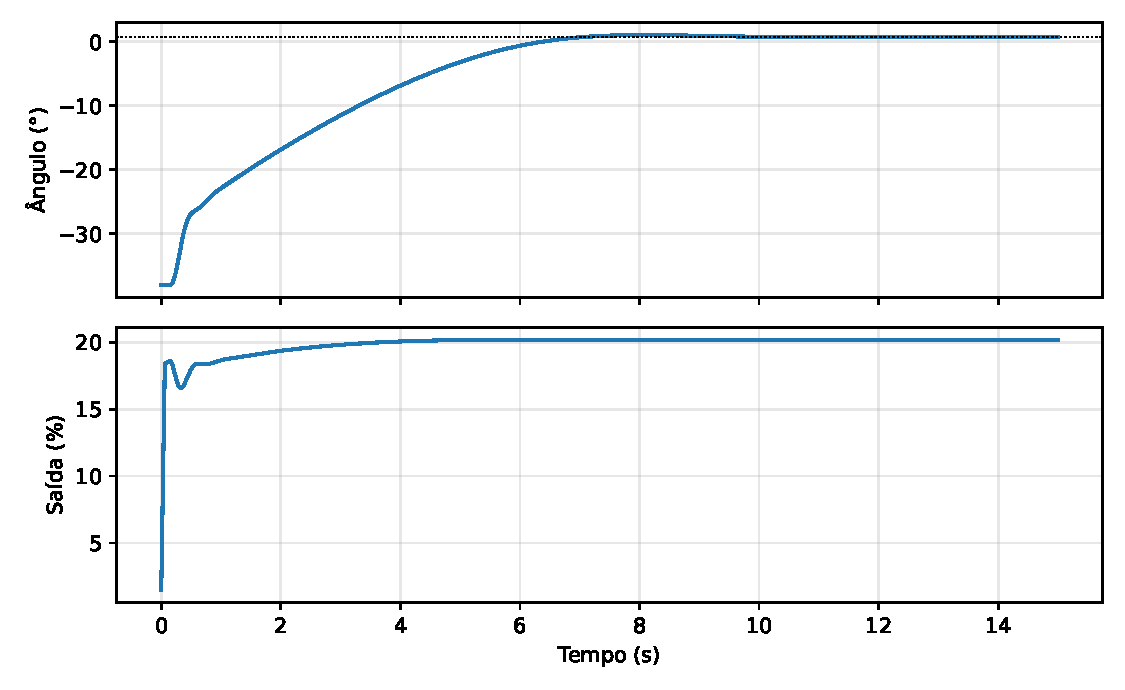
\includegraphics[width=.85\textwidth]{results/partida.pdf}
\fonte{Elaborado pelos autores (2026), simulação com a planta identificada.}
\end{figure}

\section{POR QUE O ANTI-\textit{WINDUP}}\label{sec:antiwindup}

Para isolar o efeito, a simulação segura a haste $25^\circ$ acima do alvo durante 5~s (como uma mão que a impede de se mover) e depois a solta. Durante a retenção o erro é negativo e constante; um integrador sem proteção desce sem limite e, ao soltar, a saída fica abaixo da necessária para pairar por muito tempo. Foram comparadas três versões: integrador sem proteção, integrador apenas limitado a $[0;32]\%$ e integração condicional (a do firmware), cada uma com os ganhos iniciais e com os de projeto. A simulação supõe um batente superior em $+60^\circ$, fora da faixa de interesse.
\begin{table}[htbp]
\centering\caption{Tempo para a haste voltar a $\pm2^\circ$ do alvo depois de solta (simulação).}\label{tab:windup}
\begin{tabularx}{\textwidth}{Xrr}
\hline\textbf{Estratégia} & \textbf{Ganhos iniciais} & \textbf{Ganhos de projeto}\\
 & ($1{,}0/0{,}5/0{,}15$) & ($0{,}06/0{,}05/0{,}04$)\\\hline
Sem proteção & 7,28 s & 7,34 s\\
Apenas limita o integrador & 4,90 s & 7,34 s\\
Integração condicional (firmware) & 1,01 s & 7,34 s\\\hline
\end{tabularx}
\fonte{Elaborado pelos autores (2026), com \texttt{report/simulation/sim\_1dof.py}.}
\end{table}
Com os ganhos iniciais, altos, o \textit{windup} é grave: o integrador sem proteção chega a $-41{,}5\%$ e a recuperação leva 7,3~s contra 1,0~s com a integração condicional (Figura~\ref{fig:windup}). Com os ganhos de projeto, baixos, a saída não satura na retenção e as três estratégias empatam; o anti-\textit{windup} é então uma proteção que não custa nada e passa a ser decisiva quando o ganho aumenta. O resultado também mostra que, com $K_i$ pequeno, o integrador leva cerca de 7~s para se refazer, o que é compatível com a recuperação lenta observada na bancada depois de um empurrão.
\begin{figure}[htbp]
\centering\caption{Haste retida a $+25^\circ$ por 5~s (faixa cinza) com os ganhos iniciais: efeito do \textit{windup}.}\label{fig:windup}
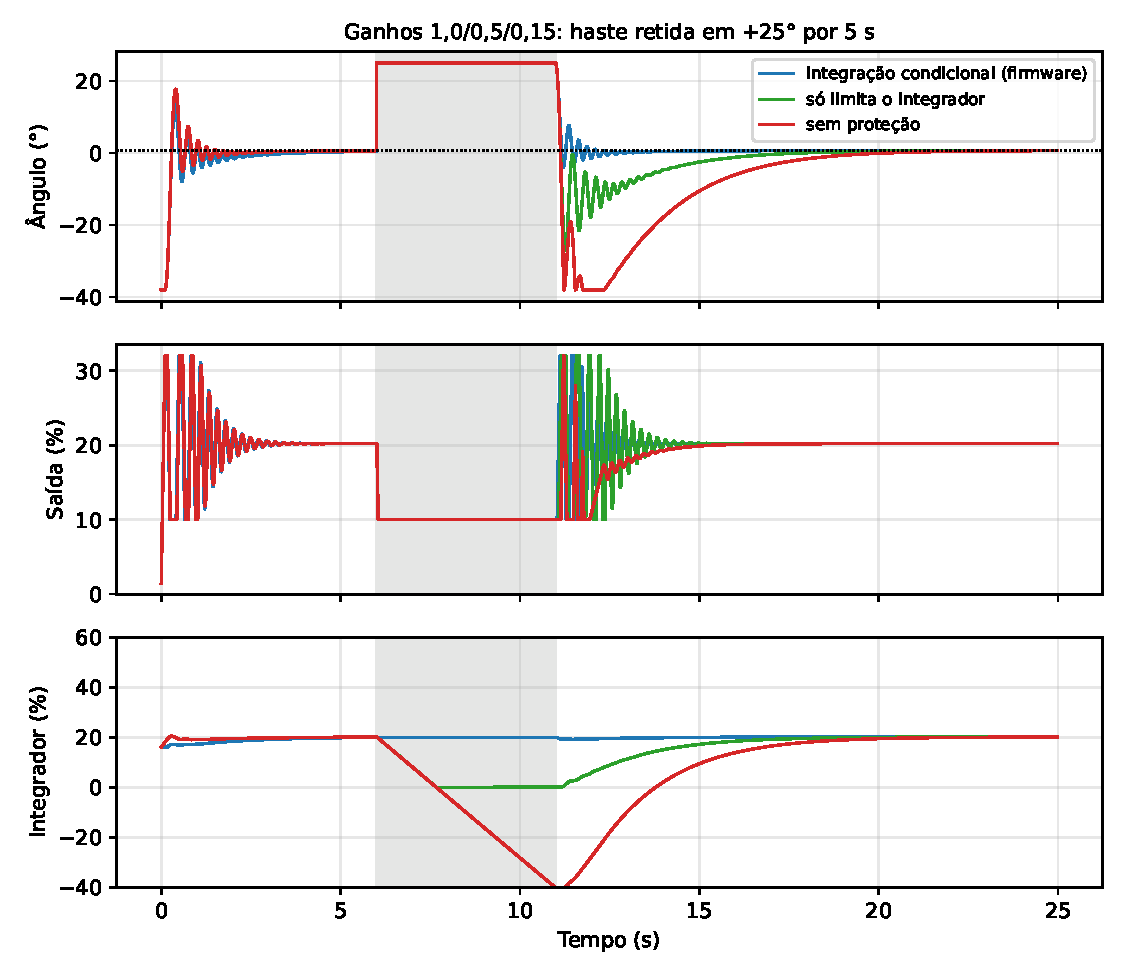
\includegraphics[width=.85\textwidth]{results/windup_ganhos_iniciais.pdf}
\fonte{Elaborado pelos autores (2026), simulação com a planta identificada.}
\end{figure}

\chapter{MATERIAIS, LIGAÇÕES E MONTAGEM}\label{cap:materiais}

\section{LISTA DE MATERIAIS}

\begin{table}[htbp]
\centering\caption{Materiais do protótipo.}\label{tab:materiais}
\begin{tabularx}{\textwidth}{p{4.3cm}X}
\hline\textbf{Item} & \textbf{Função e observações}\\\hline
Blue Pill (STM32F103C8T6) & Microcontrolador Cortex-M3 a 72~MHz, cristal de 8~MHz \cite{stm32f103ds}. Reporta 128~kB de Flash.\\
MPU6050 (módulo) & Acelerômetro e giroscópio de três eixos, ligado por I\textsuperscript{2}C no endereço 0x68 \cite{mpu6050rm}. Alimentado em 3,3~V pelo pino 3V3 da Blue Pill (o módulo aceita de 3,3 a 5~V).\\
Driver DRV8871 (módulo) & Ponte H com limite de corrente; alimentação de 6,5 a 45~V \cite{drv8871ds}. Alimentado direto pelos 12~V.\\
Motor \textit{coreless} 0720 com hélice & Motor de corrente contínua com escovas, de kit Syma: 3,7~V nominais, 7~mm de diâmetro por 20~mm de comprimento e resistência medida de cerca de 2~$\Omega$.\\
Indutor em série com o motor & Indutor toroidal de 220~$\mu$H e 3~A, com fio de cobre enrolado em núcleo toroidal (Figura~\ref{fig:fotos_potencia}), que filtra a corrente pulsada do PWM (Seção~\ref{sec:indutor}). Resistência do enrolamento menor que 0,3~$\Omega$, abaixo do que o multímetro consegue medir.\\
Fonte de 12~V & Alimenta o driver e, pelo BEC, a lógica. O consumo total estimado é inferior a 1~A (motor em torno de 0,4~A e lógica da ordem de 100~mA).\\
BEC 12~V para 5~V & Regulador chaveado que gera os 5~V da Blue Pill.\\
Chave deslizante de 3 terminais & Chave de duas posições ligada em série ao positivo de 5~V entre o BEC e a Blue Pill; um dos terminais fica sem uso. Para cima liga e para baixo desliga (Figura~\ref{fig:alimentacao}).\\
Estrutura & Base de madeira; suporte da haste, haste e caixa da eletrônica impressos em 3D. A massa não foi medida, porque o modelo foi identificado na bancada (Tabela~\ref{tab:parametros}).\\
Parafuso e porca travada & Eixo da haste na base.\\
ST-Link V2 & Gravação e leitura de diagnóstico por SWD.\\\hline
\end{tabularx}
\fonte{Elaborado pelos autores (2026).}
\end{table}

As Figuras~\ref{fig:fotos_estrutura} e~\ref{fig:fotos_potencia} mostram os componentes principais.
\begin{figure}[htbp]
\centering\caption{Estrutura e sensor: (a) suporte da haste impresso em 3D, (b) conjunto do motor com a hélice, (c) hélice e (d) MPU6050 fixado na haste.}\label{fig:fotos_estrutura}
\begin{minipage}[t]{.24\textwidth}\centering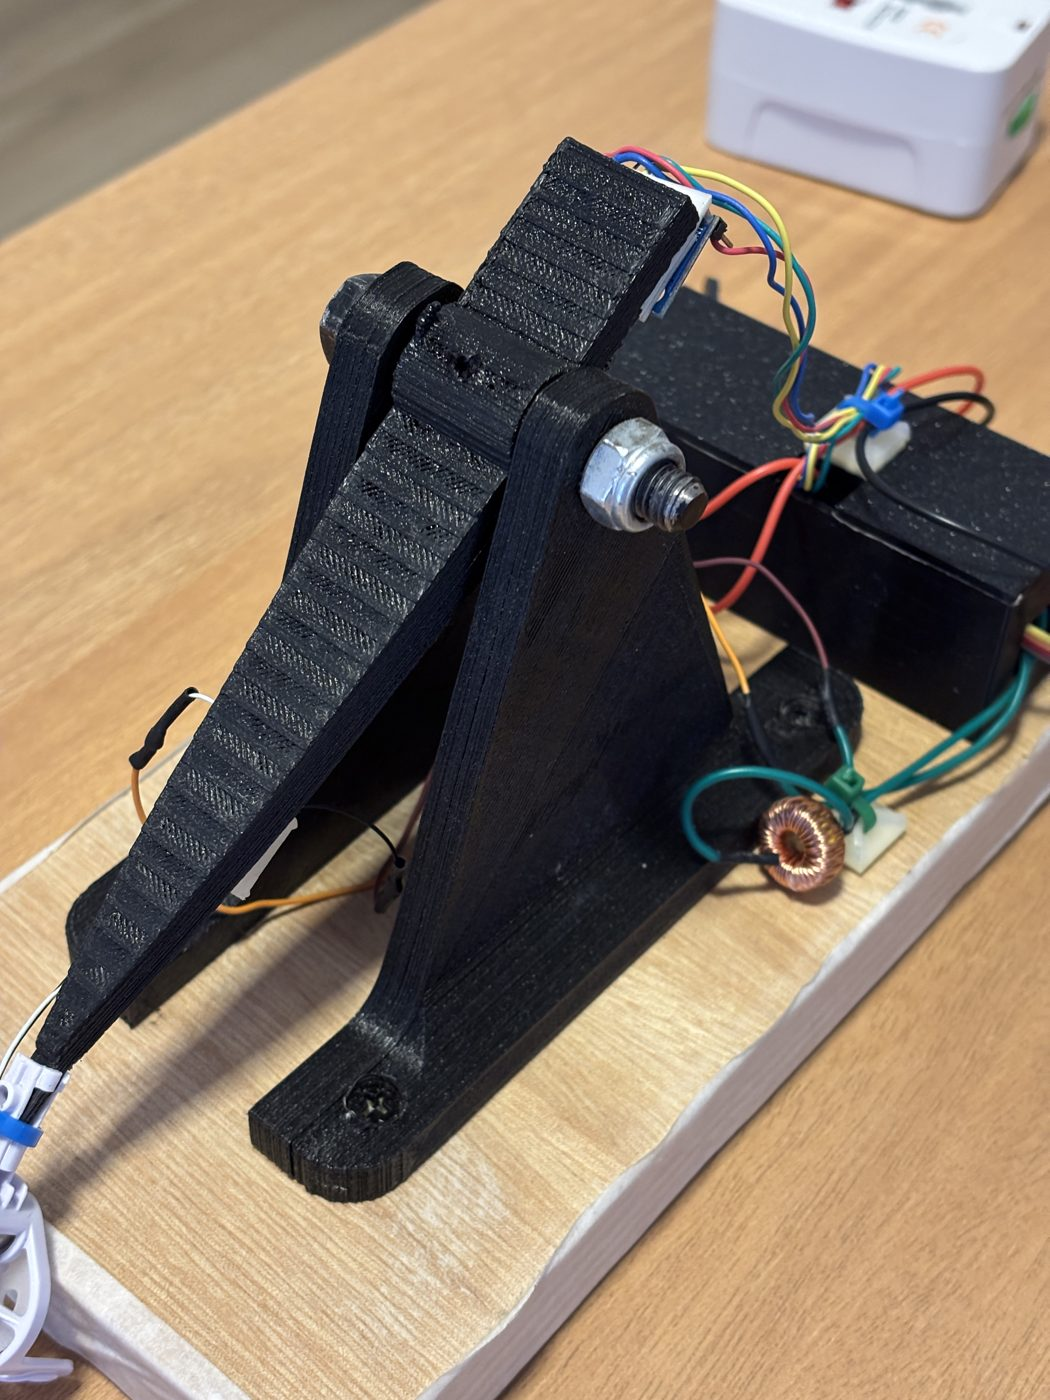
\includegraphics[width=\textwidth]{photos/base_3d.jpg}\\(a)\end{minipage}\hfill
\begin{minipage}[t]{.24\textwidth}\centering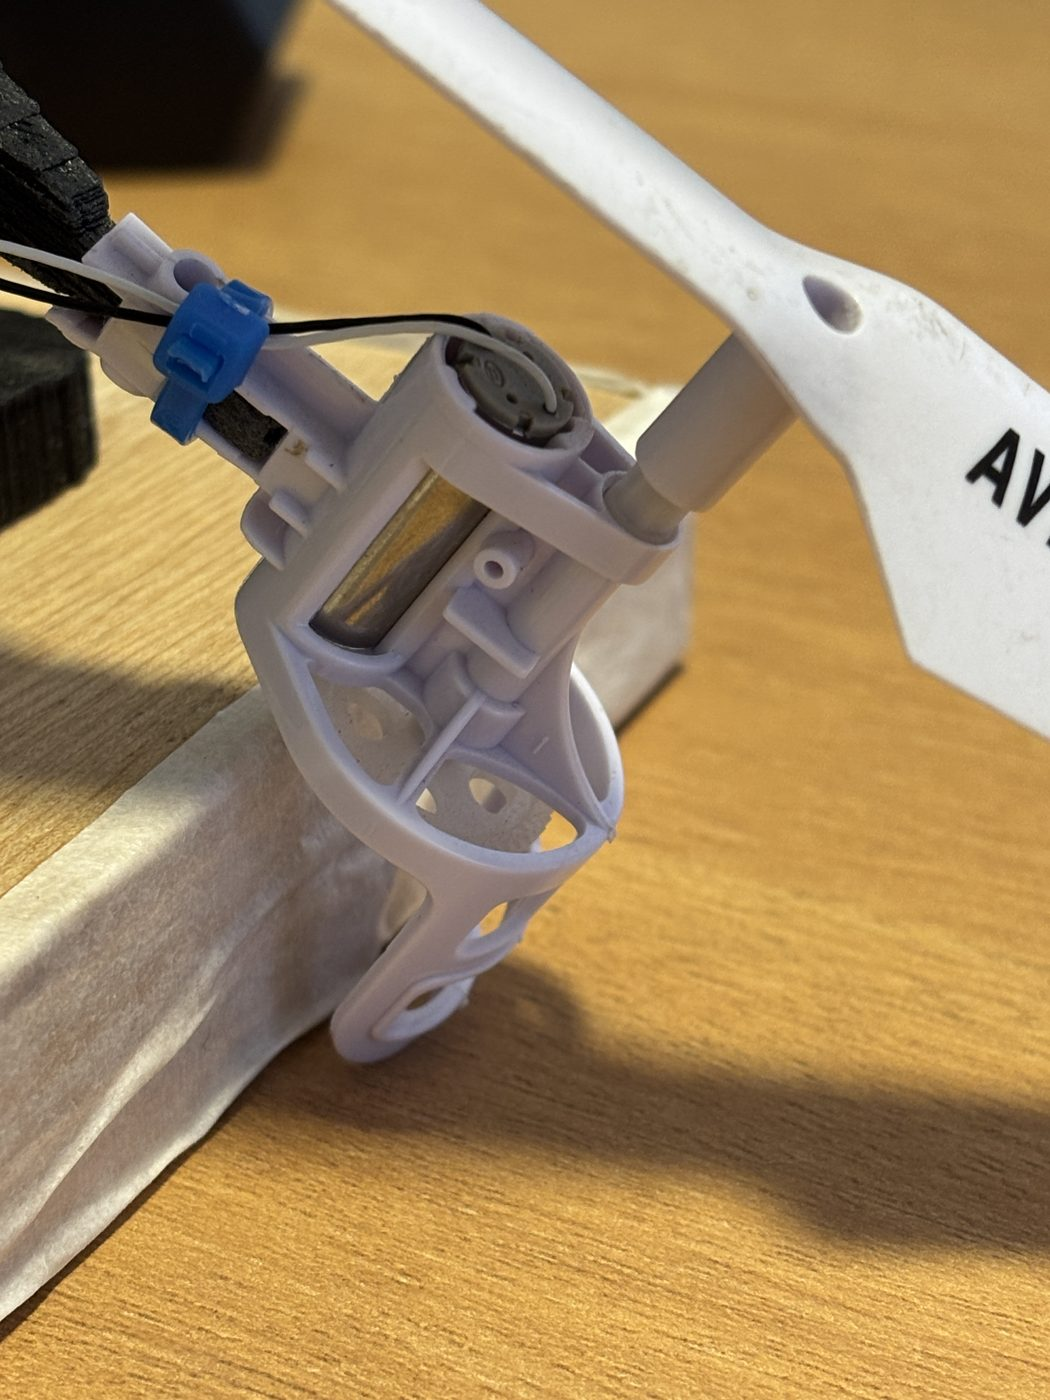
\includegraphics[width=\textwidth]{photos/motor_assembly.jpg}\\(b)\end{minipage}\hfill
\begin{minipage}[t]{.24\textwidth}\centering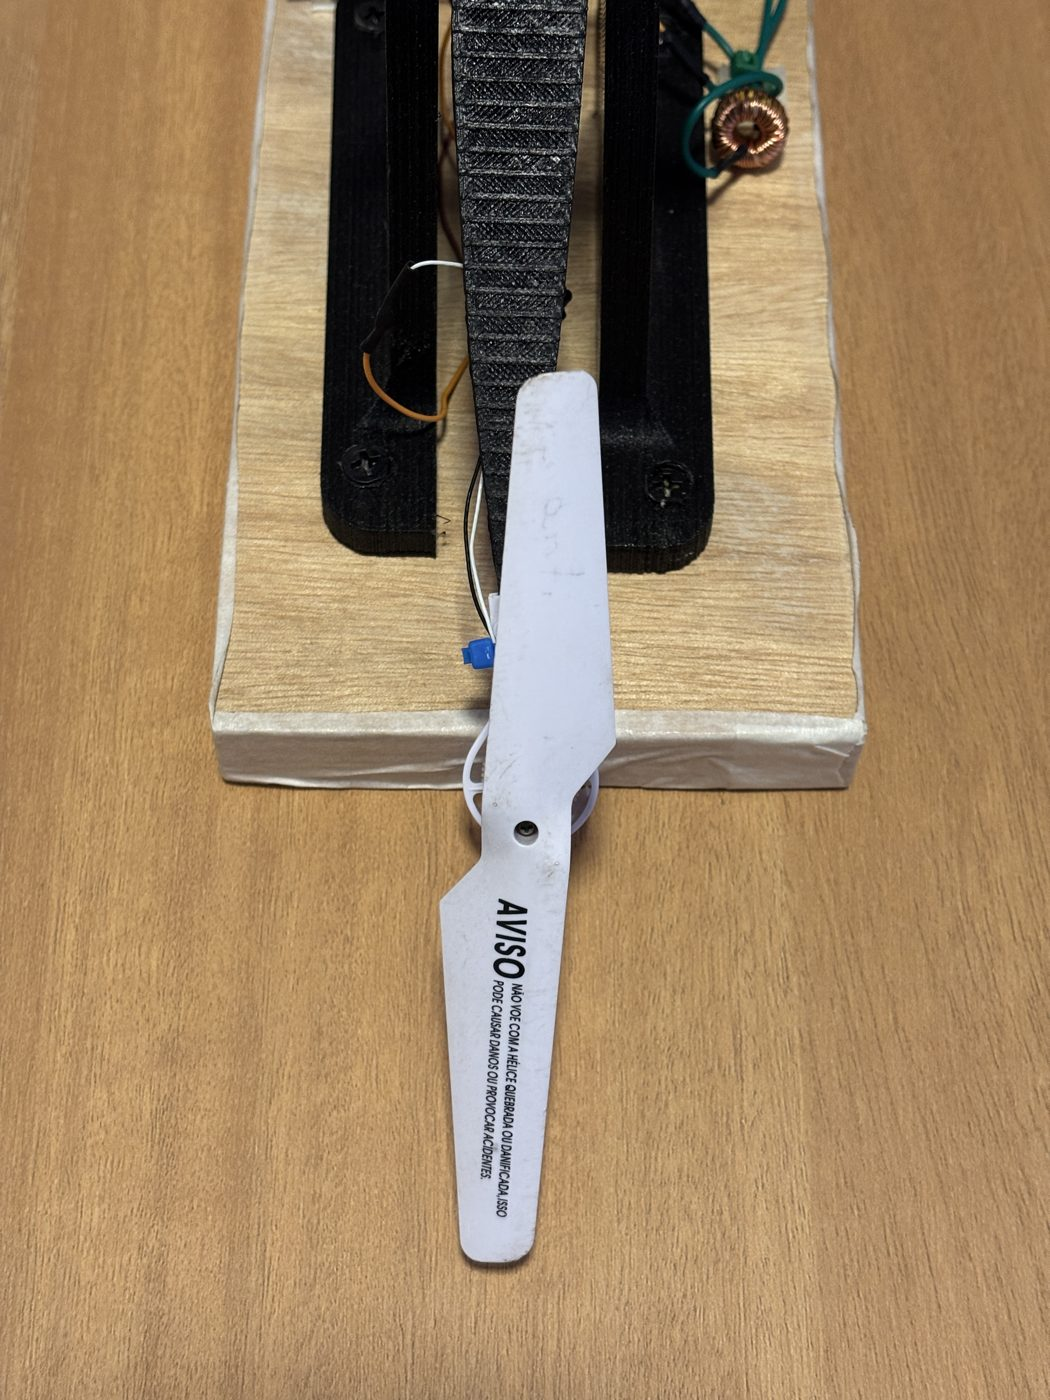
\includegraphics[width=\textwidth]{photos/propeller.jpg}\\(c)\end{minipage}\hfill
\begin{minipage}[t]{.24\textwidth}\centering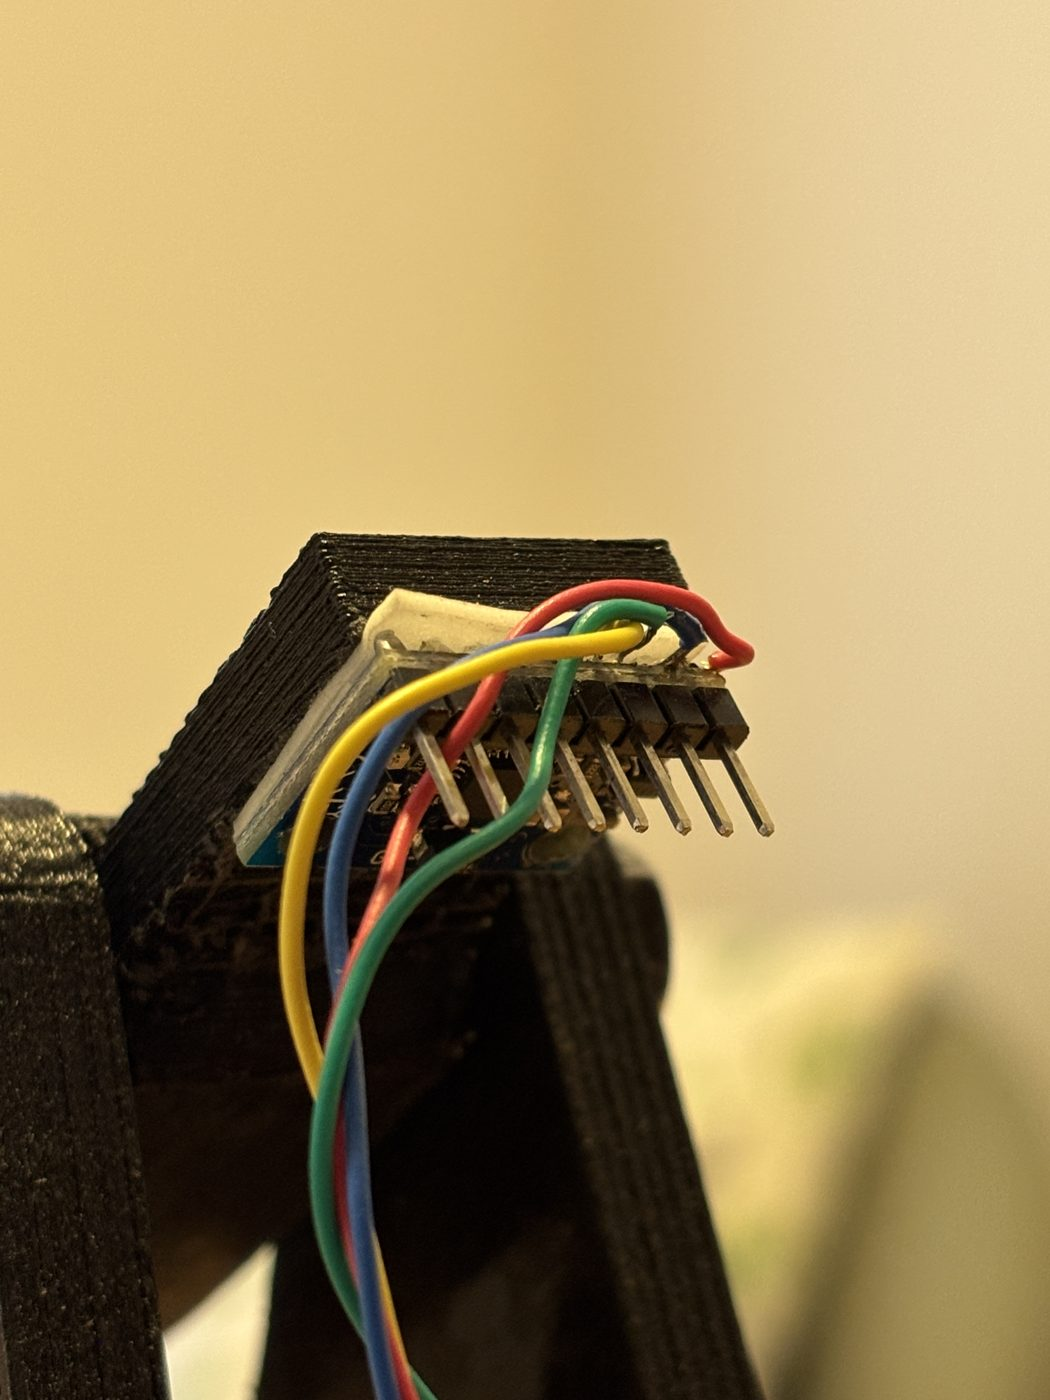
\includegraphics[width=\textwidth]{photos/mpu6050_mount.jpg}\\(d)\end{minipage}
\fonte{Elaborado pelos autores (2026).}
\end{figure}
\begin{figure}[htbp]
\centering\caption{Eletrônica e alimentação: (a) Blue Pill e driver na caixa impressa em 3D, (b) BEC com a saída de 5~V, (c) entrada de 12~V, (d) chave liga/desliga, (e) indutor toroidal de 220~$\mu$H e (f) ST-Link V2.}\label{fig:fotos_potencia}
\begin{minipage}[t]{.32\textwidth}\centering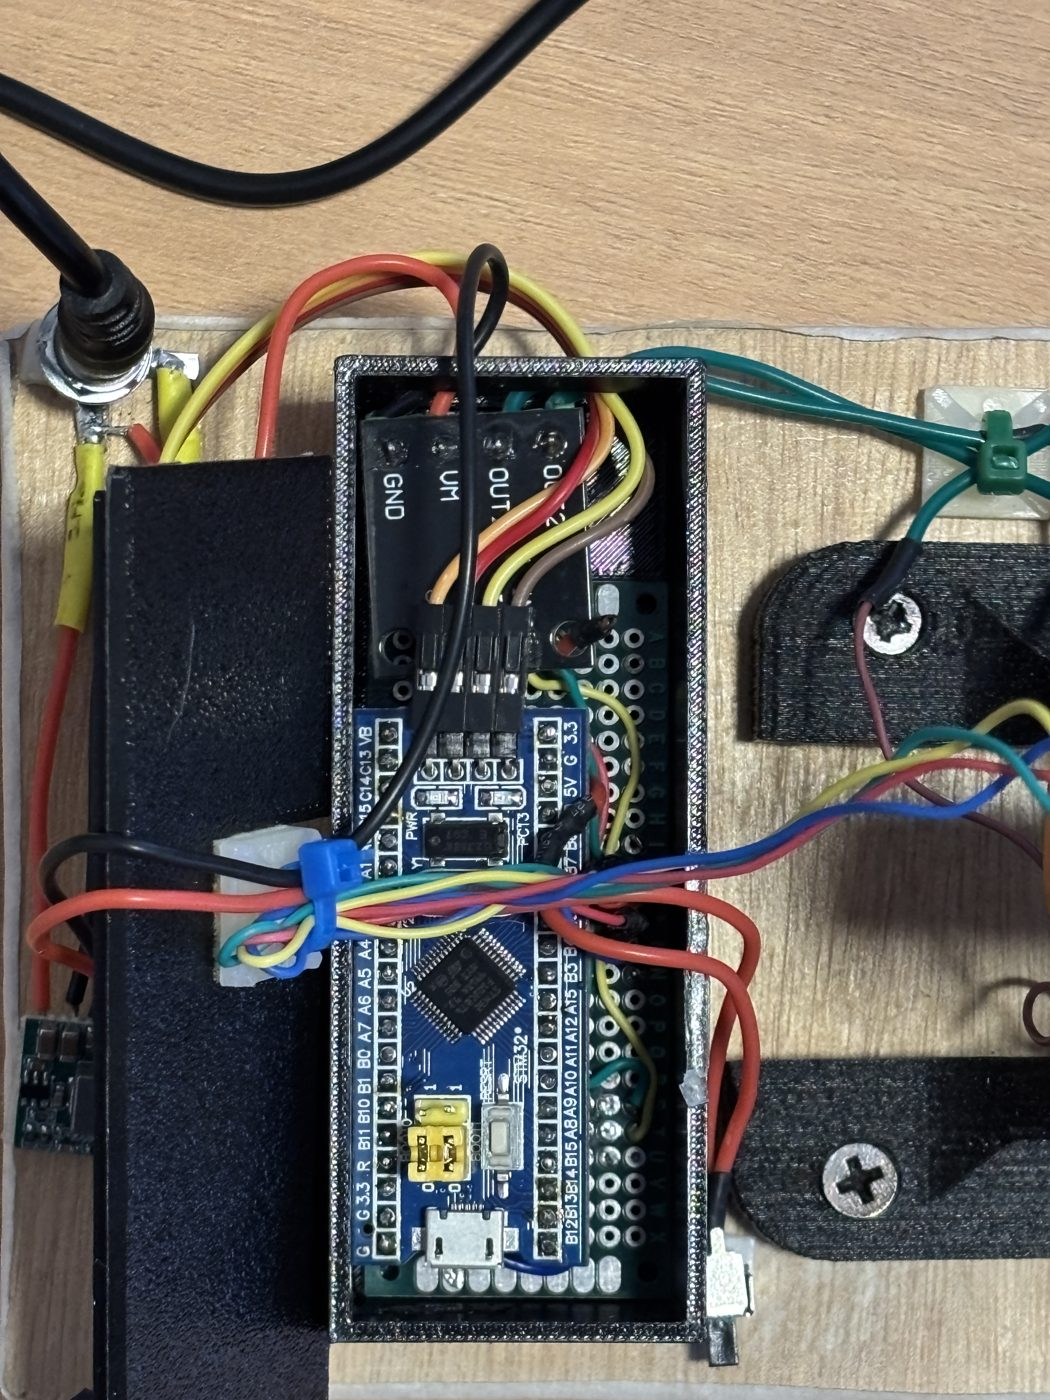
\includegraphics[width=\textwidth]{photos/stm32_driver_box.jpg}\\(a)\end{minipage}\hfill
\begin{minipage}[t]{.32\textwidth}\centering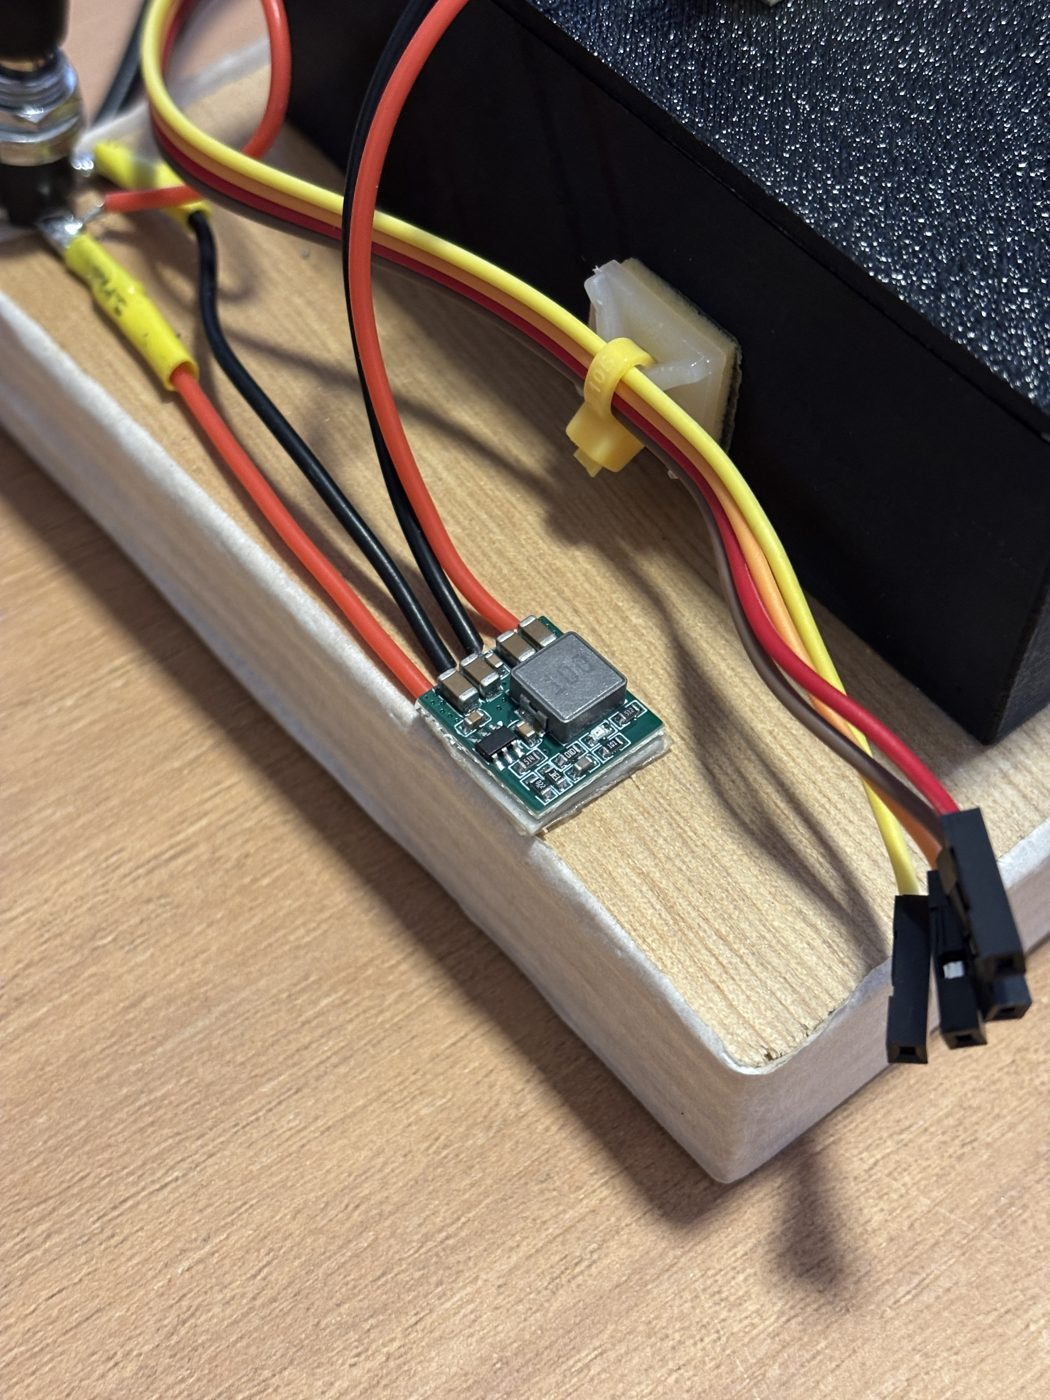
\includegraphics[width=\textwidth]{photos/bec_5v_output.jpg}\\(b)\end{minipage}\hfill
\begin{minipage}[t]{.32\textwidth}\centering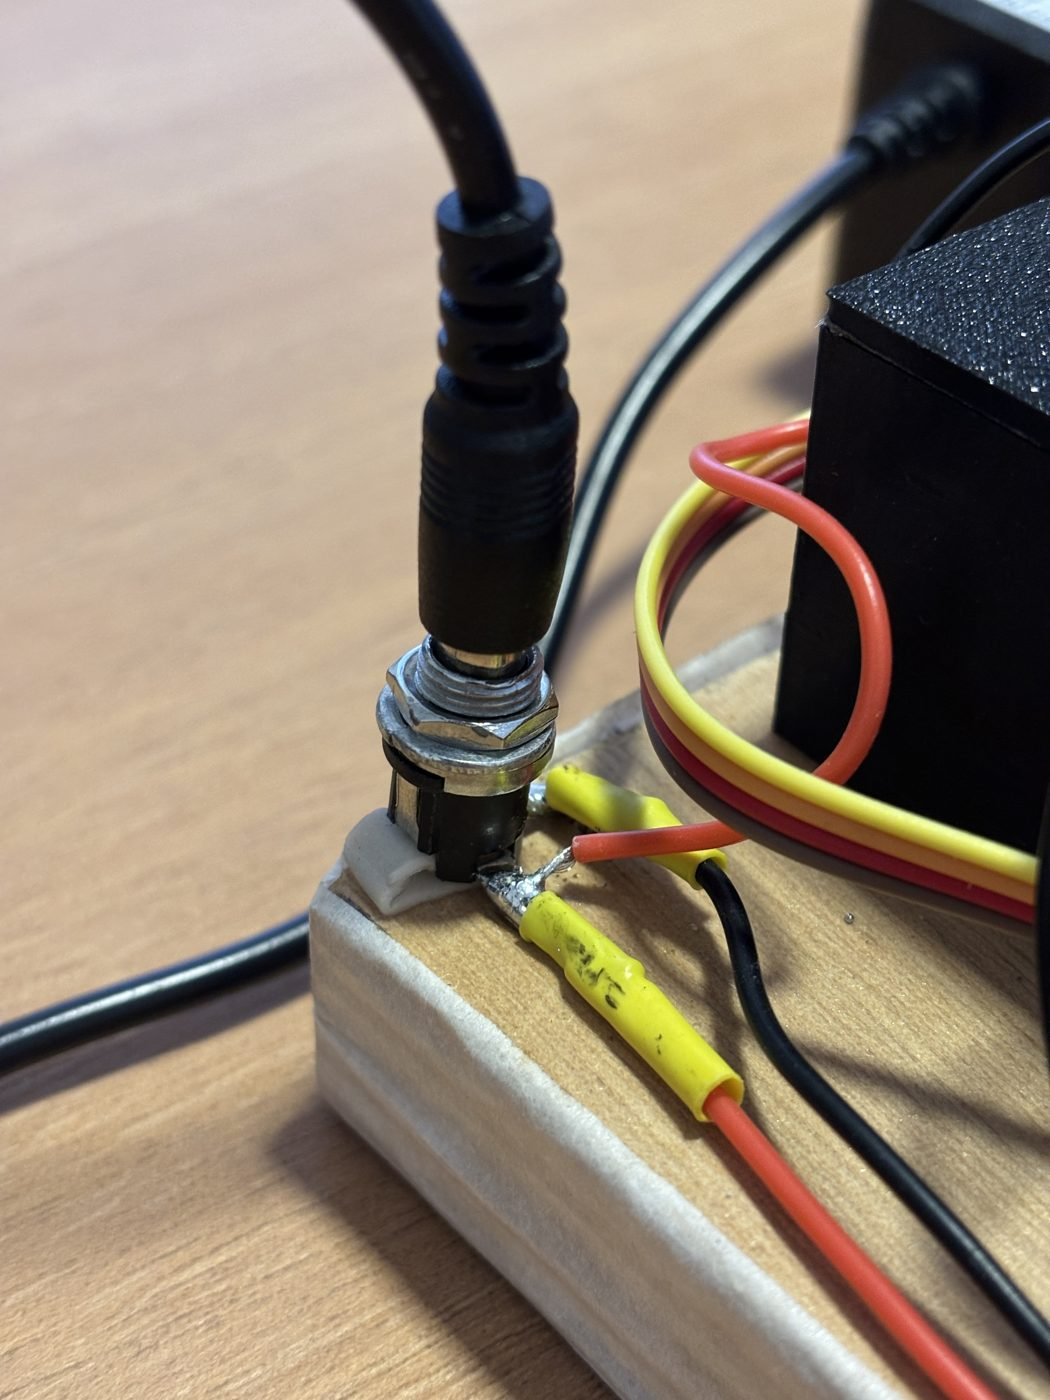
\includegraphics[width=\textwidth]{photos/input_12v.jpg}\\(c)\end{minipage}\\[6pt]
\begin{minipage}[t]{.32\textwidth}\centering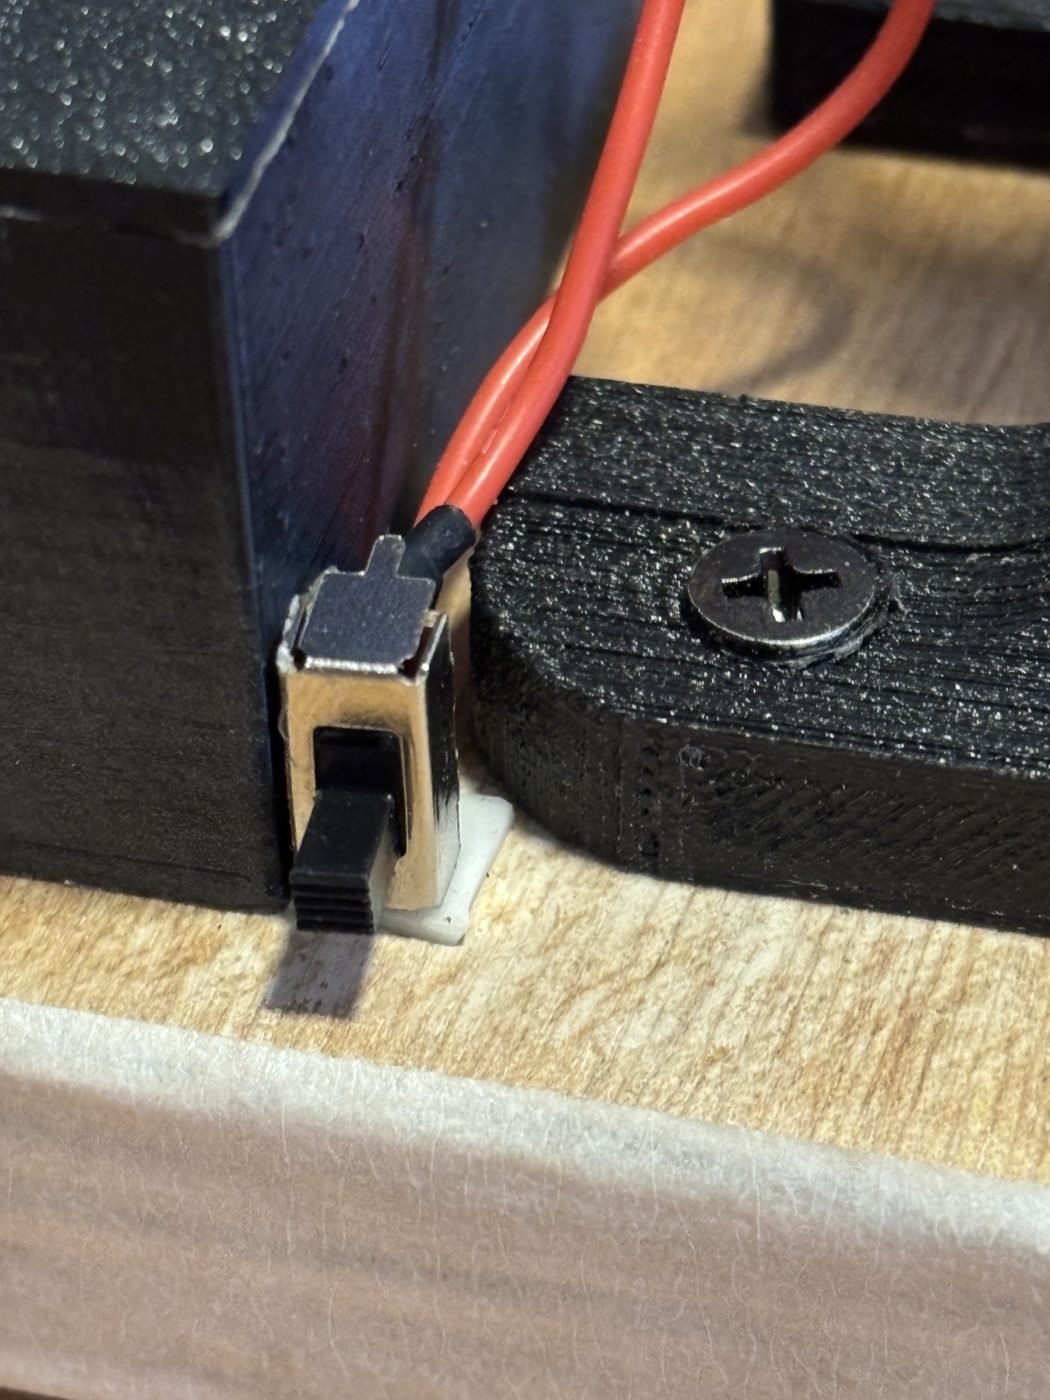
\includegraphics[width=\textwidth]{photos/power_switch.jpg}\\(d)\end{minipage}\hfill
\begin{minipage}[t]{.32\textwidth}\centering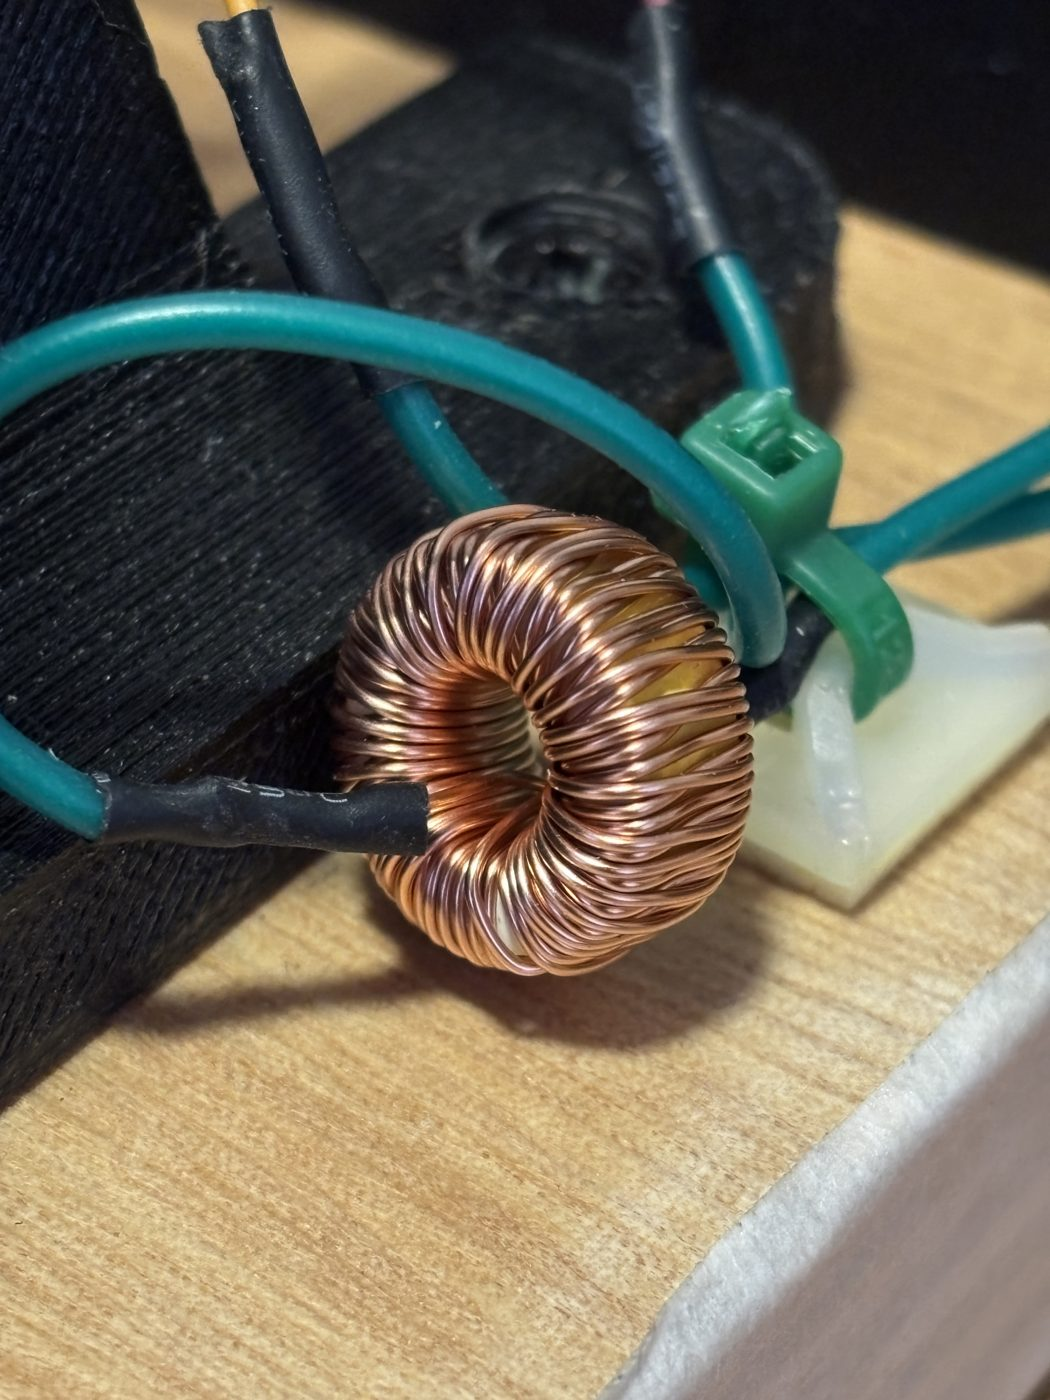
\includegraphics[width=\textwidth]{photos/inductor_toroid.jpg}\\(e)\end{minipage}\hfill
\begin{minipage}[t]{.32\textwidth}\centering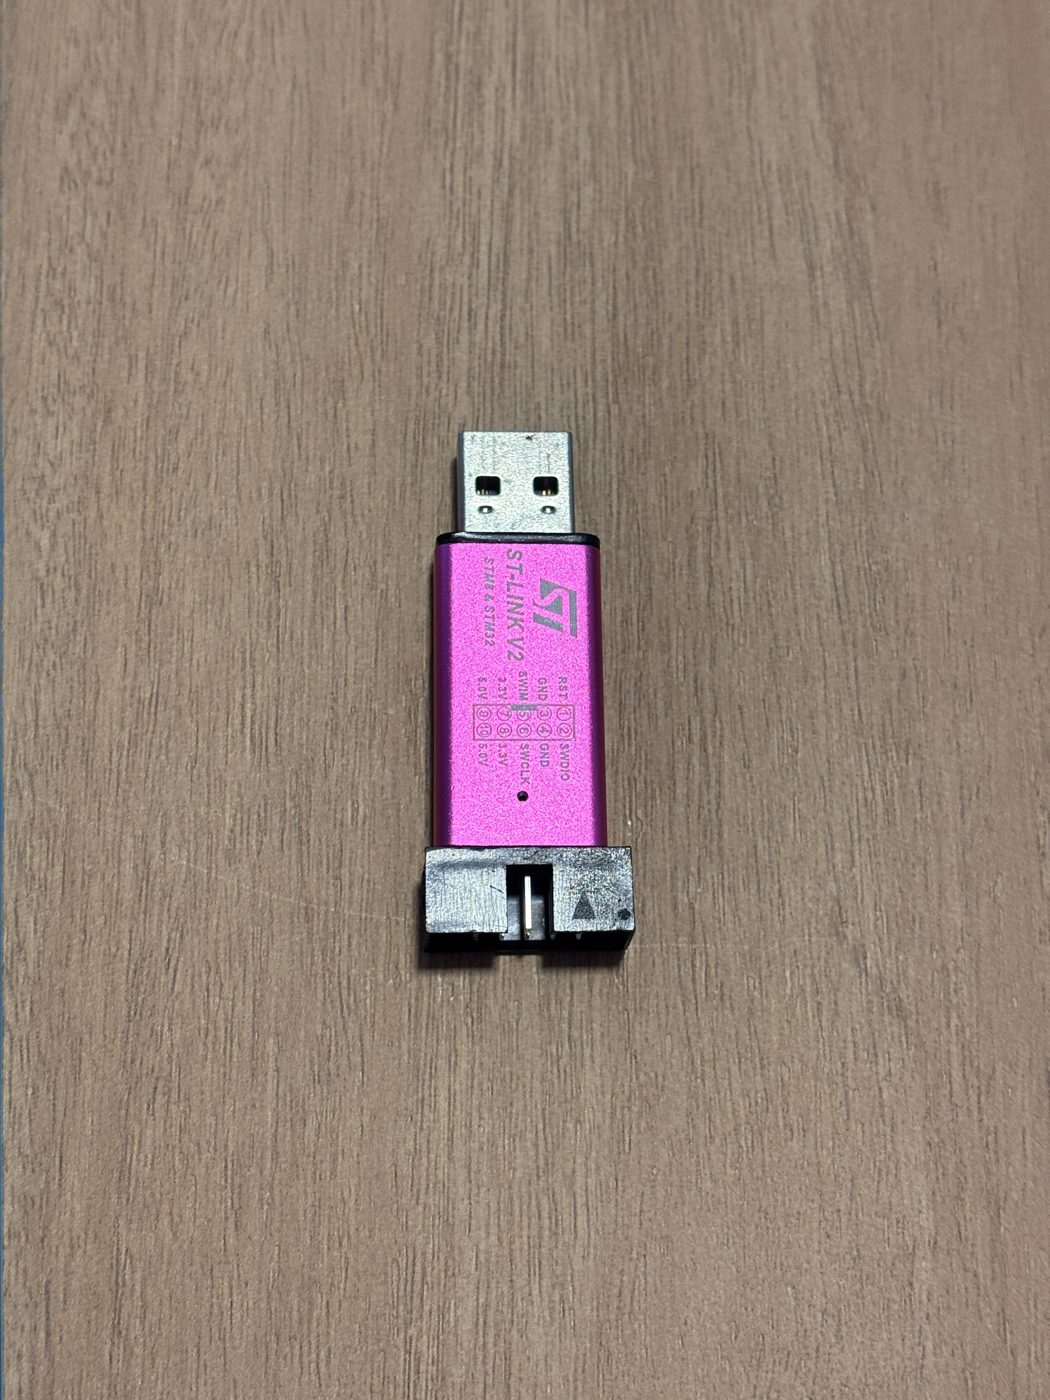
\includegraphics[width=\textwidth]{photos/stlink.jpg}\\(f)\end{minipage}
\fonte{Elaborado pelos autores (2026).}
\end{figure}

\section{ALIMENTAÇÃO}

A fonte de 12~V alimenta o driver diretamente (VM) e, em paralelo, o BEC. A saída de 5~V do BEC passa pela chave deslizante e chega ao pino 5V da Blue Pill; o regulador de 3,3~V da placa alimenta o MPU6050. Todos os terras são comuns. A Figura~\ref{fig:alimentacao} resume o esquema.
\begin{figure}[htbp]
\centering\caption{Distribuição de alimentação.}\label{fig:alimentacao}
\begin{tikzpicture}[node distance=9mm and 11mm,box/.style={draw,align=center,minimum height=10mm,font=\small,text width=2.6cm},arr/.style={-{Latex},thick}]
\node[box] (fonte) {Fonte\\12~V};
\node[box,right=of fonte] (bec) {BEC\\12~V$\to$5~V};
\node[box,right=of bec] (chave) {Chave\\deslizante};
\node[box,right=of chave] (bp) {Blue Pill\\(3,3~V)};
\node[box,below=of bp] (mpu) {MPU6050};
\node[box,below=of bec] (drv) {DRV8871\\(VM = 12~V)};
\node[box,below=of chave] (mot) {Indutor\\+ motor};
\draw[arr] (fonte)--(bec); \draw[arr] (bec)--(chave); \draw[arr] (chave)--(bp);
\draw[arr] (bp)--node[right,font=\scriptsize]{3,3~V}(mpu);
\draw[arr] (fonte.south)|-(drv.west);
\draw[arr] (drv)--(mot);
\end{tikzpicture}
\fonte{Elaborado pelos autores (2026).}
\end{figure}
A chave interrompe somente os 5~V da lógica; o driver continua ligado aos 12~V. Sem os 5~V, o microcontrolador desliga, as entradas do driver ficam sem sinal e o motor para. Assim, a chave faz o papel de liga/desliga do controle, enquanto a fonte de 12~V permanece conectada.

\section{LIGAÇÕES}

\begin{quadro}[htbp]
\centering
\caption{Mapa de interfaces do protótipo.}\label{tab:pinos}
\begin{tabularx}{\textwidth}{|p{1.8cm}|p{2.5cm}|p{3.4cm}|X|}
\hline
\textbf{STM32} & \textbf{Componente} & \textbf{Sinal} & \textbf{Função}\\ \hline
PA9 & DRV8871 & IN2 / TIM1 CH2 & nível alto fixo enquanto a saída é maior que zero (sentido em que a hélice empurra a haste para cima)\\
PA8 & DRV8871 & IN1 / TIM1 CH1 & PWM do motor: com PA9 em nível alto, o motor é acionado enquanto PA8 está baixo e freia quando está alto\\
PB6 & MPU6050 & SCL / I\textsuperscript{2}C1 & relógio do barramento, 400~kHz\\
PB7 & MPU6050 & SDA / I\textsuperscript{2}C1 & dados do barramento\\
PA2 / PA3 & Interface serial & USART2 TX/RX & comandos e telemetria, 115200 8N1 (opcional)\\
PC13 & LED da placa & GPIO & estado: calibrando, rodando, sem sensor\\
PA13 / PA14 & ST-Link & SWDIO / SWCLK & gravação e diagnóstico\\
GND & todos & referência & terra comum\\ \hline
\end{tabularx}
\fonte{Elaborado pelos autores (2026), conforme \texttt{topicos2.ioc}.}
\end{quadro}
A Figura~\ref{fig:esquema} mostra a fiação por pino. O motor fica entre OUT1 e OUT2 do driver, com o indutor em série no fio de OUT1, perto do driver e fora da haste. Não há capacitor externo na entrada VM do driver. Os componentes internos dos módulos MPU6050 e DRV8871, como resistores de \textit{pull-up}, não aparecem no desenho.
\begin{figure}[htbp]
\centering\caption{Diagrama de ligações do protótipo.}\label{fig:esquema}
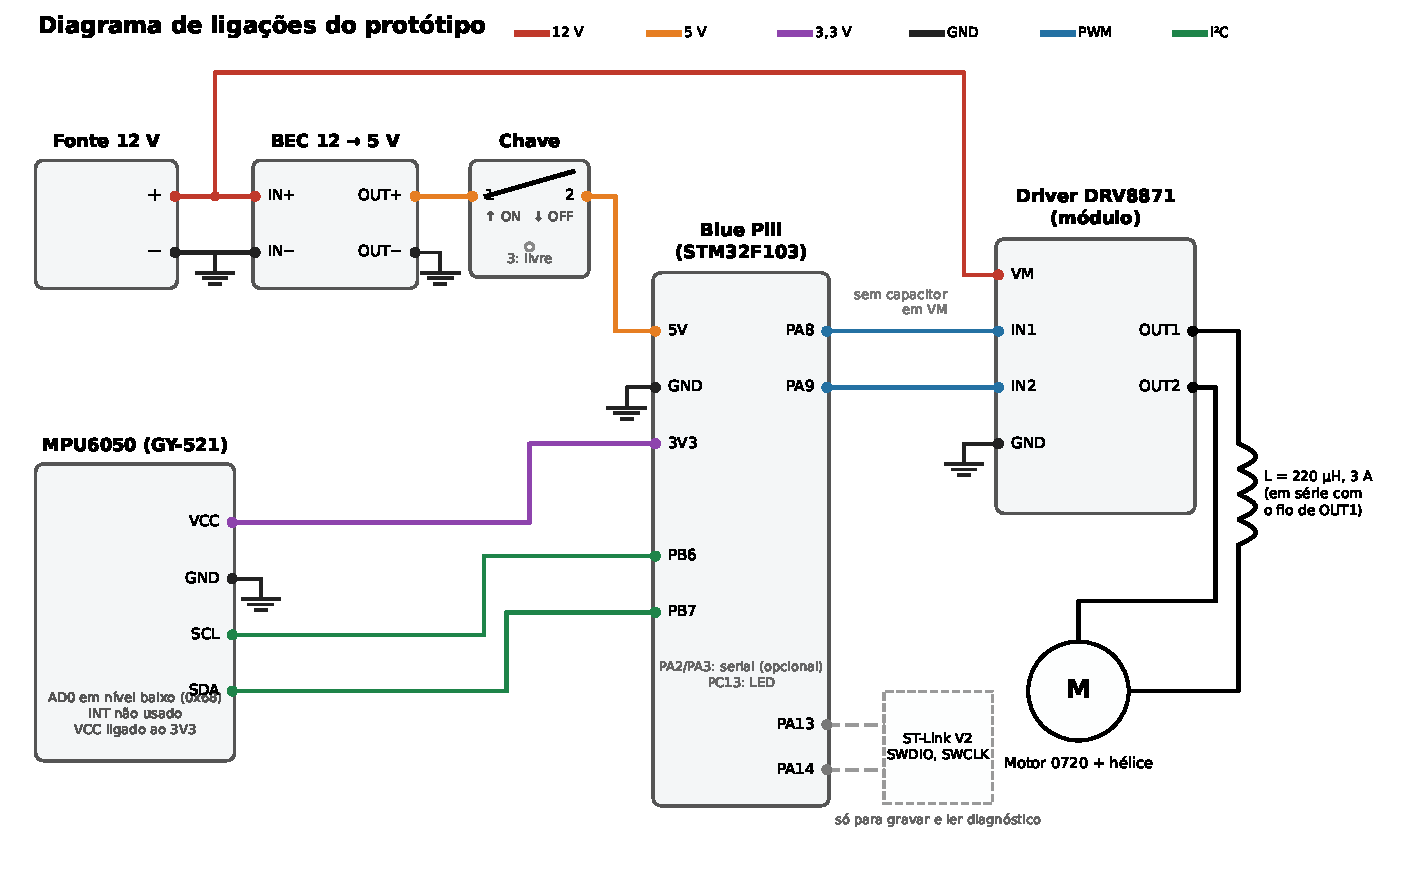
\includegraphics[width=\textwidth]{hardware/esquema_ligacoes.pdf}
\fonte{Elaborado pelos autores (2026), conforme \texttt{topicos2.ioc} e a montagem do protótipo.}
\end{figure}
Um mau contato no cabo do motor chegou a manter a haste parada com saída máxima durante 8~s; por isso todas as ligações foram soldadas.

\section{MONTAGEM MECÂNICA}

A Blue Pill e o driver ficam dentro da caixa fechada. A haste é presa ao suporte por um parafuso com porca travada, que forma o eixo de rotação. O motor com a hélice fica em uma ponta da haste e o MPU6050 na outra, preso com fita dupla face. O sensor está montado de cabeça para baixo e a haste gira em torno do eixo Y dele; o firmware compensa com uma soma de $180^\circ$ ao ângulo (Capítulo~\ref{cap:desenvolvimento}). O sentido de empuxo foi confirmado visualmente na bancada.

\section{PROTÓTIPO FINAL}

A estrutura final tem uma base de madeira, o suporte da haste impresso em 3D, a haste com o motor e a hélice em uma ponta e o MPU6050 na outra, e uma caixa impressa em 3D que abriga a Blue Pill e o driver, com a chave liga/desliga na lateral. As Figuras~\ref{fig:final_cima} a~\ref{fig:final_tras} mostram o protótipo montado.
\begin{figure}[htbp]
\centering\caption{Protótipo final, visto de cima.}\label{fig:final_cima}
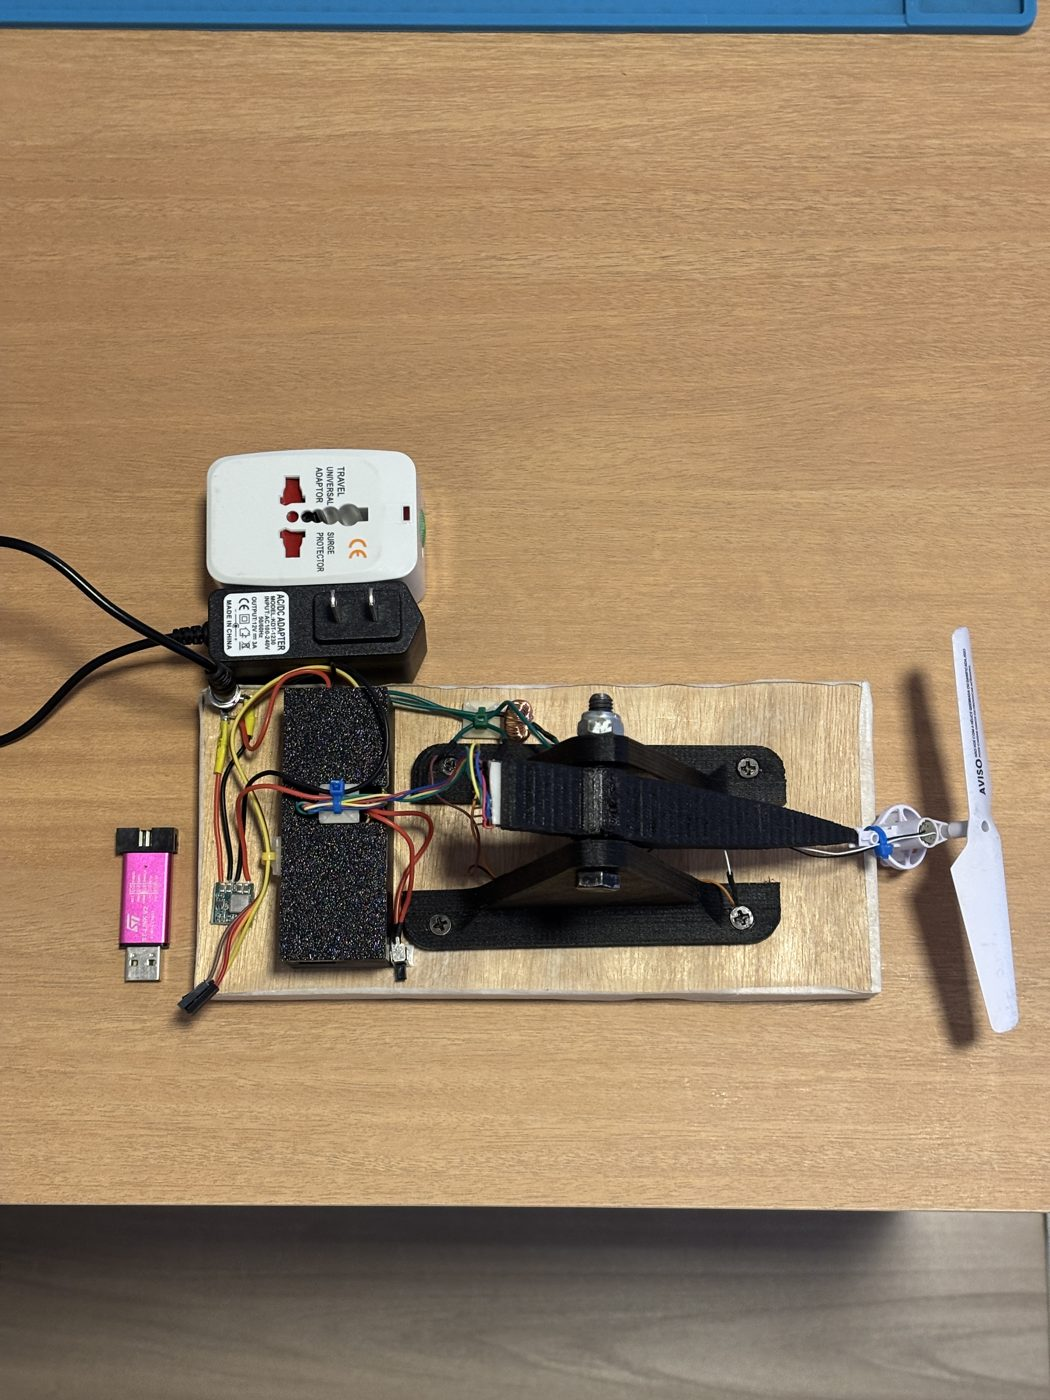
\includegraphics[height=.42\textheight]{photos/final_top.jpg}
\fonte{Elaborado pelos autores (2026).}
\end{figure}
\begin{figure}[htbp]
\centering\caption{Protótipo final: (a) visto de frente e (b) visto de lado.}\label{fig:final_lado}
\begin{minipage}[t]{.48\textwidth}\centering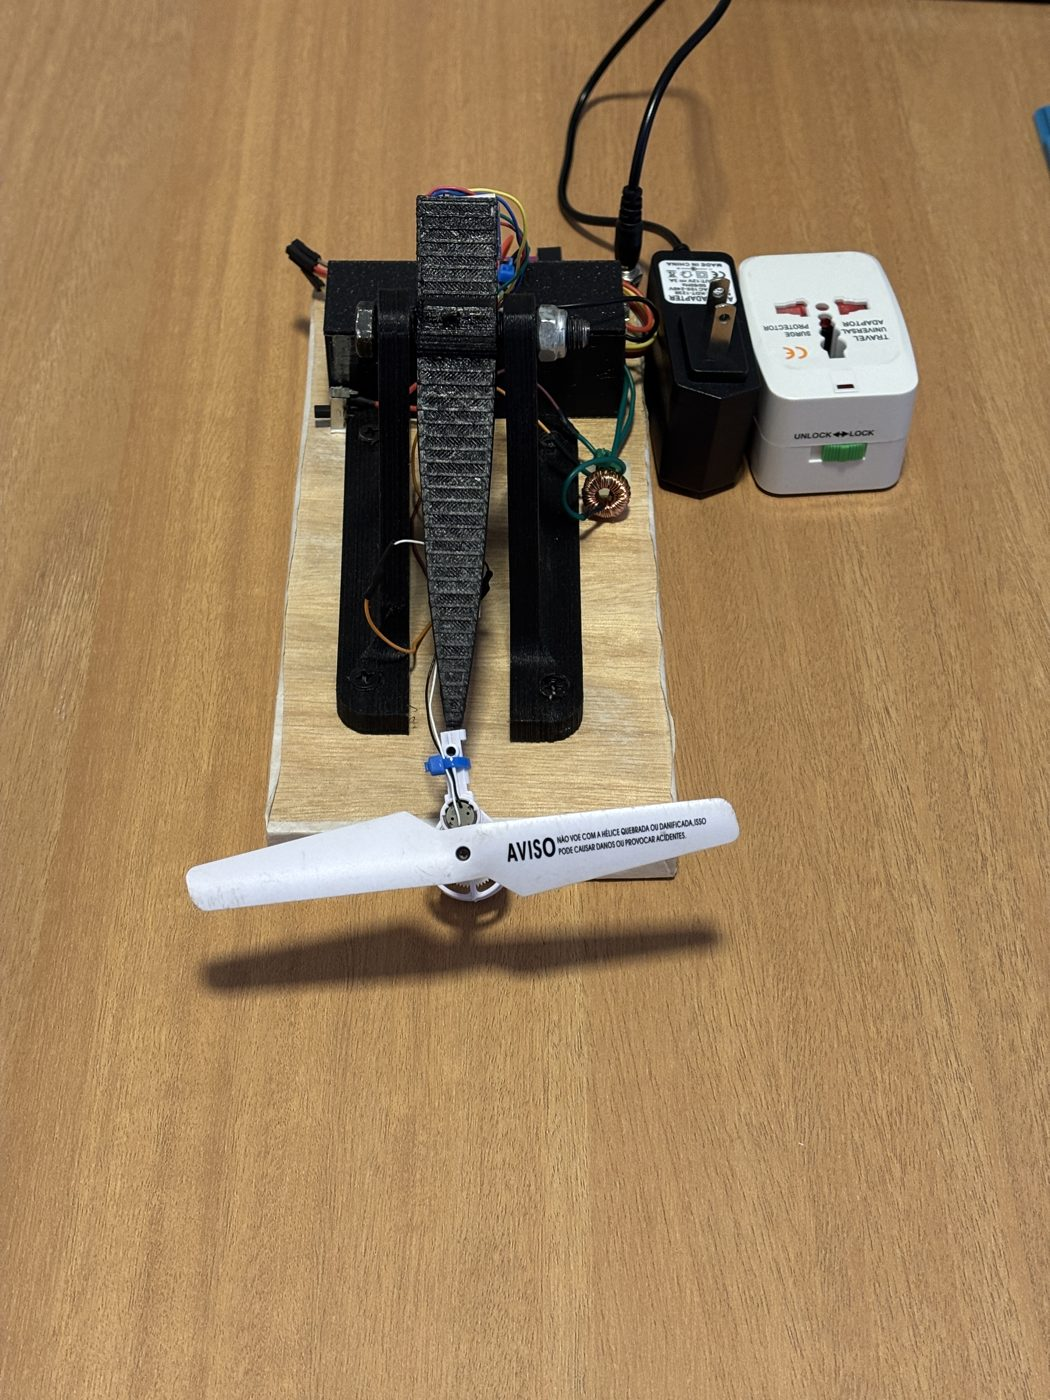
\includegraphics[height=.34\textheight]{photos/final_front.jpg}\\(a)\end{minipage}\hfill
\begin{minipage}[t]{.48\textwidth}\centering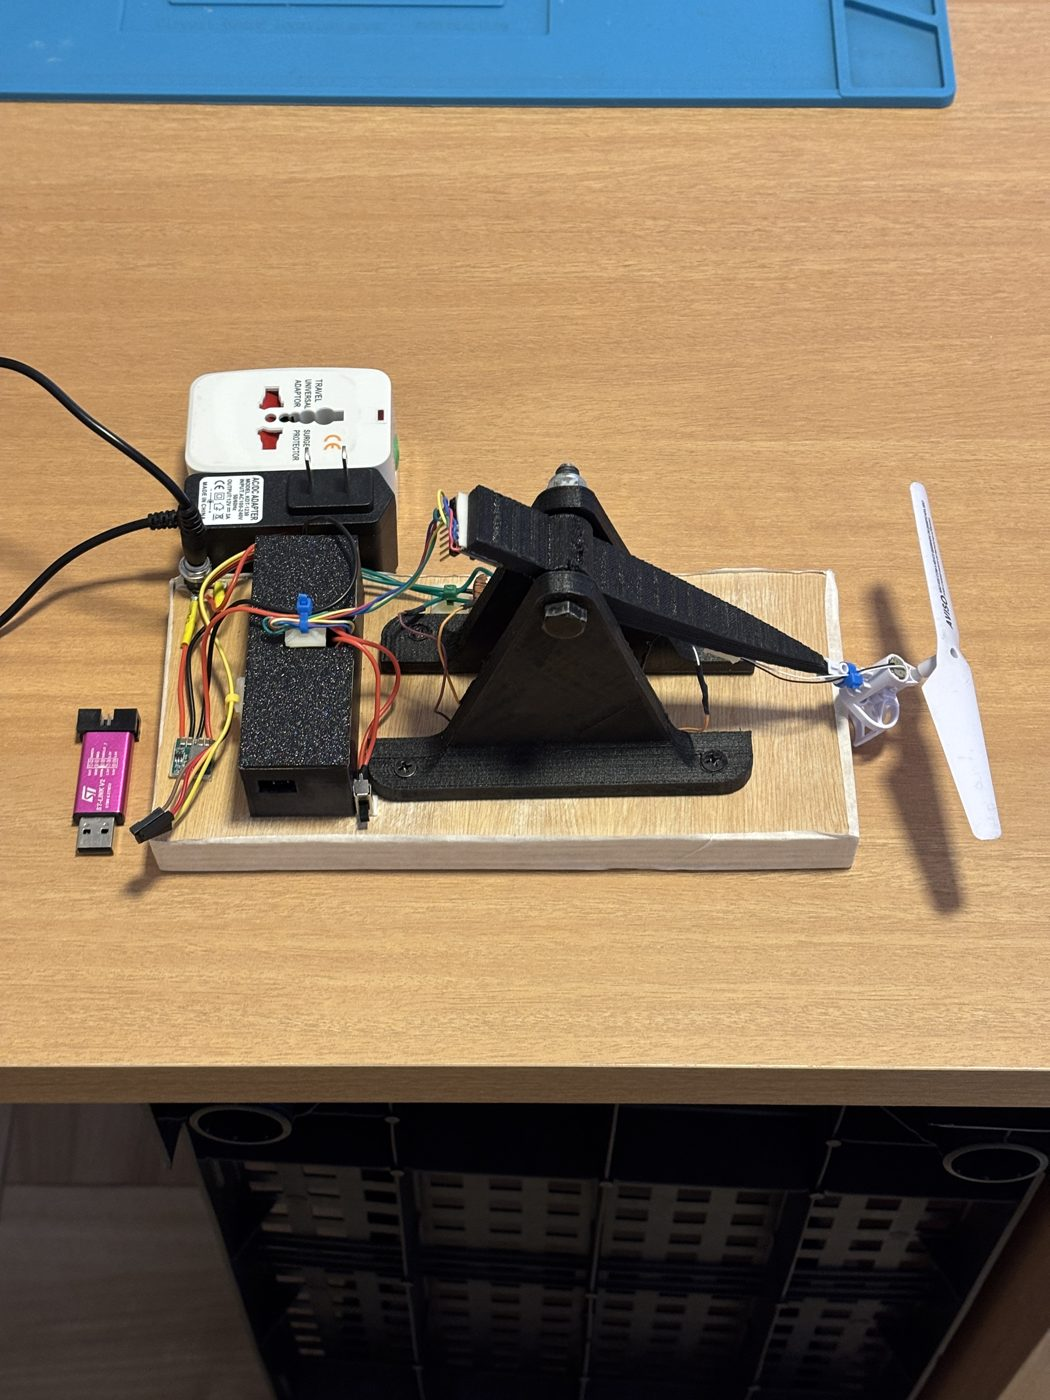
\includegraphics[height=.34\textheight]{photos/final_side_1.jpg}\\(b)\end{minipage}
\fonte{Elaborado pelos autores (2026).}
\end{figure}
\begin{figure}[htbp]
\centering\caption{Protótipo final, visto de trás, com a fonte, o adaptador, a caixa da eletrônica e o ST-Link.}\label{fig:final_tras}
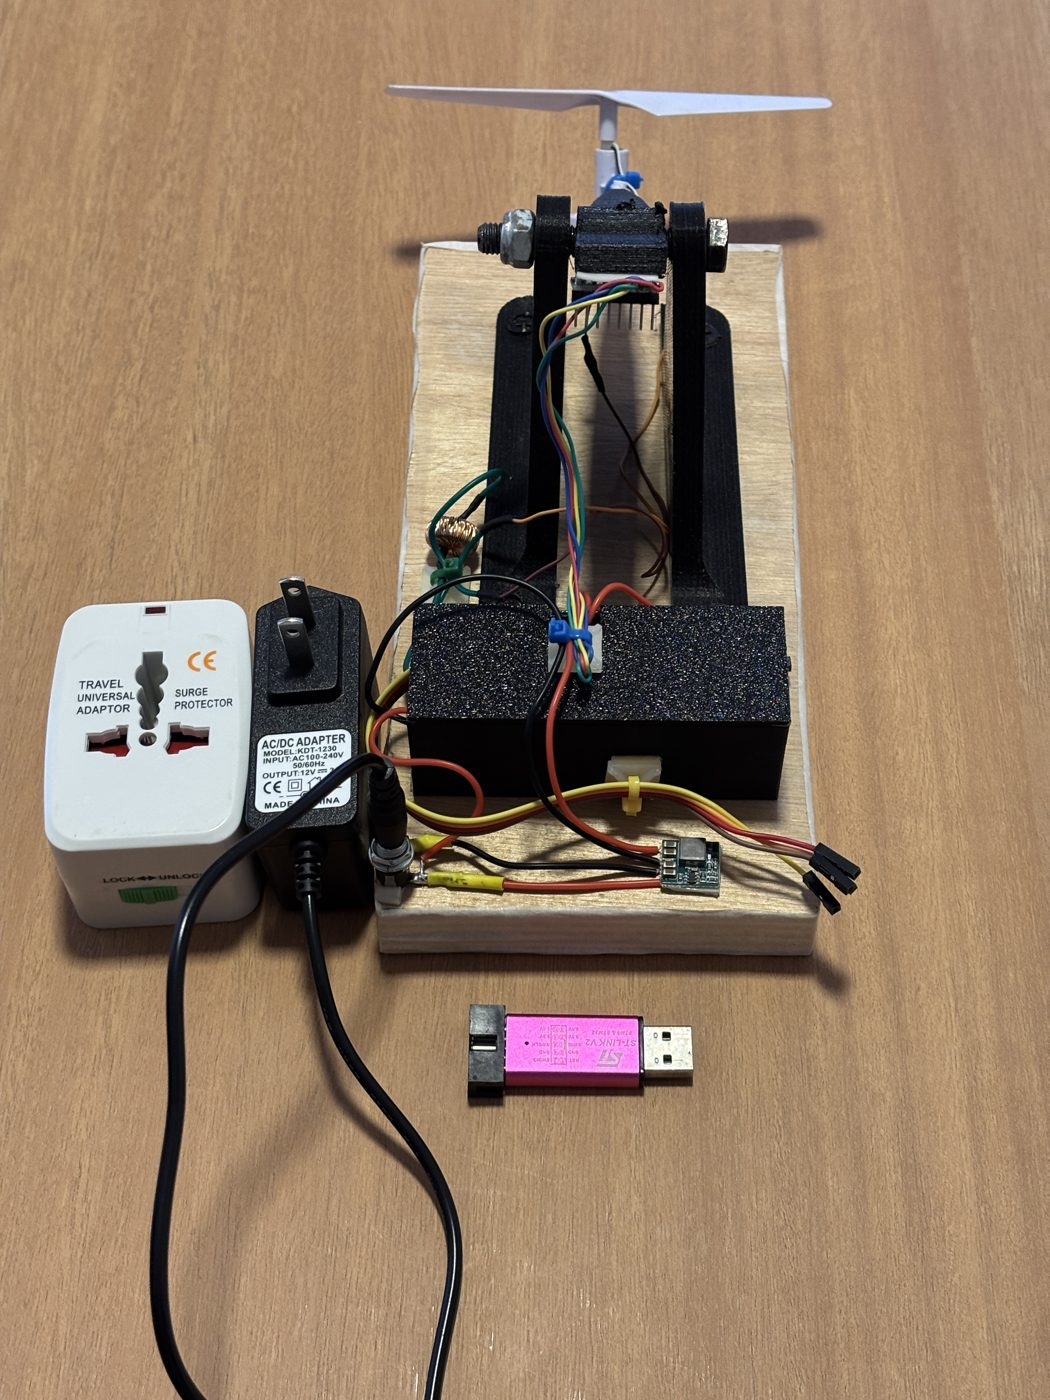
\includegraphics[height=.42\textheight]{photos/final_back.jpg}
\fonte{Elaborado pelos autores (2026).}
\end{figure}
\fotofinal{final_rodando}{Protótipo final com a haste estabilizada, em funcionamento.}{fig:final_rodando}

\section{ESTUDO DA POTÊNCIA DO MOTOR}\label{sec:potencia}

O motor tem tensão nominal de 3,7~V e é alimentado por 12~V através do driver. A tensão média é controlada pelo PWM, limitado a 32\%, o que dá cerca de 3,8~V médios (12~V $\times$ 0,32), próximo do nominal. O DRV8871 desarma por sobrecorrente entre 3,7 e 6,4~A e religa depois de 3~ms, e não funciona abaixo de 6,5~V \cite{drv8871ds}; por isso não dá para alimentá-lo com os 3,7~V do motor. Daí os 12~V com PWM baixo. A Seção~\ref{sec:indutor} mostra o efeito colateral dessa escolha.

\chapter{DESENVOLVIMENTO DO FIRMWARE}\label{cap:desenvolvimento}

Este capítulo reúne o necessário para reproduzir o firmware: ferramentas, configuração do microcontrolador, organização em módulos, tarefas e objetos do FreeRTOS.

\section{FERRAMENTAS E VERSÕES}

\begin{table}[htbp]
\centering\caption{Ambiente de desenvolvimento.}\label{tab:versoes}
\begin{tabularx}{\textwidth}{lX}
\hline\textbf{Item} & \textbf{Versão}\\\hline
IDE / CubeMX & STM32CubeIDE 2.2.0 (projeto gerado com o CubeMX integrado)\\
Pacote do chip & STM32Cube FW\_F1 V1.8.7 (HAL e CMSIS)\\
Compilador & GNU Tools for STM32 14.3.rel1 (\texttt{arm-none-eabi-gcc} 14.3.1), \textit{newlib-nano}\\
FreeRTOS & Kernel V10.3.1, porta ARM\_CM3, \textit{heap\_4}; camada CMSIS-RTOS V2 usada apenas pelo código gerado\\
Gravação e leitura & STM32CubeProgrammer 2.23.0 com ST-Link V2 (SWD)\\
Simulação e análise & Python 3, NumPy, Matplotlib; GCC no computador para \texttt{firmware/tests/sim\_control.c}\\
Verificação de regras & \texttt{firmware/tools/misra\_check.sh} (MISRA C:2012)\\\hline
\end{tabularx}
\fonte{Elaborado pelos autores (2026).}
\end{table}

\section{CONFIGURAÇÃO DO STM32}

\begin{table}[htbp]
\centering\caption{Configuração dos periféricos (\texttt{topicos2.ioc}).}\label{tab:config}
\begin{tabularx}{\textwidth}{lX}
\hline\textbf{Periférico} & \textbf{Configuração}\\\hline
Clock & HSE de 8~MHz, PLL $\times9$: SYSCLK e HCLK de 72~MHz, APB1 de 36~MHz, APB2 de 72~MHz\\
TIM1 (PA8, PA9) & PWM nos canais 1 e 2; o CubeMX configura 20~kHz e \texttt{Motor\_Init} recalcula para 100~kHz (prescaler 0, ARR 719)\\
TIM2 & Prescaler 7199 e período 49: estouro a 200~Hz (5~ms), com interrupção; libera o semáforo de controle\\
I2C1 (PB6, PB7) & Modo rápido, 400~kHz\\
USART2 (PA2, PA3) & 115200 bit/s, 8N1; recepção por interrupção\\
Base de tempo da HAL & TIM4 (o SysTick fica com o FreeRTOS)\\
FreeRTOS & \textit{tick} de 1~kHz, preempção ligada, \textit{heap} de 8192~bytes, 56 níveis de prioridade, \textit{mutexes} e semáforos contadores ligados\\
NVIC & Grupo de prioridades 4 (4 bits de preempção); TIM2 e USART2 em prioridade 5, igual ao limite \texttt{configMAX\_SYSCALL\_INTERRUPT\_PRIORITY}; PendSV e SysTick em 15\\\hline
\end{tabularx}
\fonte{Elaborado pelos autores (2026).}
\end{table}
O MPU6050 é configurado por \texttt{Mpu\_Init}: relógio pelo PLL do giroscópio, filtro digital de 44~Hz, taxa de saída de 200~Hz, giroscópio de $\pm1000^\circ$/s e acelerômetro de $\pm16$~g. As escalas largas evitam saturar o sensor na queda da haste ($>500^\circ$/s) e na vibração da hélice.

\section{ORGANIZAÇÃO EM MÓDULOS}

O código escrito pelo grupo fica em \texttt{firmware/Modules/}, separado do código gerado pelo CubeMX (\texttt{firmware/Core/}). Cada módulo tem uma responsabilidade; o módulo de controle não depende de hardware nem de RTOS, o que permite executá-lo no computador.
\begin{table}[htbp]
\centering\caption{Módulos do firmware.}\label{tab:modulos}
\begin{tabularx}{\textwidth}{lX}
\hline\textbf{Módulo} & \textbf{Conteúdo}\\\hline
\texttt{app/} & \texttt{app\_config.h}: todos os ajustes em um só lugar; \texttt{app.c}: tarefa de controle, semáforo, \textit{mutex} de dados e acesso aos dados compartilhados\\
\texttt{sensor/} & \texttt{mpu6050.c}: leitura por I\textsuperscript{2}C e conversão de escalas; \texttt{angle\_filter.c}: filtro complementar\\
\texttt{control/} & \texttt{pid.c}: PID com derivada na medida e anti-\textit{windup}; \texttt{control.c}: filtro da derivada e rampa da saída\\
\texttt{motor/} & \texttt{motor.c}: PWM do DRV8871 (frequência, modo de freio, limite)\\
\texttt{serial/} & \texttt{serial.c}: comandos, telemetria, LED, tarefas de comando e telemetria, fila e \textit{mutex} da UART\\
\texttt{debug/} & \texttt{debug.c}: contadores e registro circular na RAM, lidos pelo ST-Link sem serial\\\hline
\end{tabularx}
\fonte{Elaborado pelos autores (2026).}
\end{table}

Todo o código escrito pelo grupo segue o mesmo padrão. As funções públicas são documentadas com Doxygen, em português, e os trechos feitos à mão (PID, filtro, registradores do MPU6050, PWM do DRV8871) citam a fonte consultada. Os nomes indicam o módulo, o tipo e a unidade, como em \texttt{Motor\_Set}, \texttt{Pid\_t} e \texttt{angle\_deg}. Os módulos foram conferidos com as regras do MISRA C:2012; os desvios são todos de regras \textit{advisory}: uso direto de \texttt{float} (Dir.~4.6), conversões de endereço feitas pelas macros da HAL (Reg.~11.4) e funções globais exigidas pela HAL e pelo CubeMX (Reg.~8.7).

Todos os ajustes do projeto ficam em um único arquivo, \texttt{app\_config.h}. As Tabelas~\ref{tab:parametros_fw}, \ref{tab:parametros_motor} e~\ref{tab:parametros_ctrl} explicam cada valor e o motivo da escolha.
\begin{table}[H]
\centering\caption{Parâmetros de amostragem e sensor (\texttt{app\_config.h}).}\label{tab:parametros_fw}
\begin{tabularx}{\textwidth}{>{\raggedright\arraybackslash}p{3.7cm}>{\raggedright\arraybackslash}p{2.3cm}X}
\hline\textbf{Parâmetro} & \textbf{Valor} & \textbf{Significado e motivo}\\\hline
\texttt{CTRL\_PERIOD\_S} & 0,005 s & Período do laço de controle (200~Hz), gerado pelo TIM2. É cerca de doze vezes menor que o atraso do empuxo.\\
\texttt{IMU\_AXIS\_X} & 0 & A haste gira em torno do eixo Y do sensor: o ângulo vem de \texttt{atan2(-ax, az)} e a velocidade, do giroscópio Y.\\
\texttt{ANGLE\_OFFSET\_DEG} & 180$^\circ$ & Soma ao ângulo medido para compensar o sensor montado de cabeça para baixo, de modo que $0^\circ$ seja a horizontal.\\
\texttt{COMP\_TAU\_S} & 2,0 s & Constante do filtro complementar com o motor parado: em escalas de tempo menores que ela, vale o giroscópio; em maiores, o acelerômetro.\\
\texttt{COMP\_TAU\_FLIGHT\_S} & 30 s & Constante do filtro com o motor ligado. Em voo o acelerômetro é ruidoso, mas não deriva; uma correção muito lenta segura a deriva do giroscópio sem deixar o ruído passar.\\
\texttt{ACC\_FLIGHT\_GATE\_DEG} & 25$^\circ$ & Em voo, descarta a leitura do acelerômetro que difira da estimativa por mais que isso (as amostras de $-48^\circ$ a $+46^\circ$ vistas em voo).\\
\hline
\end{tabularx}
\fonte{Elaborado pelos autores (2026).}
\end{table}

\begin{table}[H]
\centering\caption{Parâmetros do motor (\texttt{app\_config.h}).}\label{tab:parametros_motor}
\begin{tabularx}{\textwidth}{>{\raggedright\arraybackslash}p{3.7cm}>{\raggedright\arraybackslash}p{2.3cm}X}
\hline\textbf{Parâmetro} & \textbf{Valor} & \textbf{Significado e motivo}\\\hline
\texttt{MOTOR\_SIGN} & $-1$ & Escolhe IN2 (PA9) como a entrada que aciona o motor, o sentido em que a hélice empurra a haste para cima. O motor nunca gira ao contrário.\\
\texttt{MOTOR\_PWM\_HZ} & 100~kHz & Frequência do PWM. É alta para que a corrente do motor, que tem indutância muito baixa, fique lisa. Em 1 e 20~kHz o driver desarmou; em 200~kHz a haste não equilibrou.\\
\texttt{MOTOR\_SLOW\_DECAY} & 1 & Entre os pulsos, o motor é freado em vez de solto. Com o indutor, a corrente fica lisa e a tensão média no motor é a saída em porcentagem vezes 12~V.\\
\texttt{OUT\_LIMIT\_PCT} & 32\% & Teto da saída. Com 12~V equivale a cerca de 3,8~V médios, perto dos 3,7~V nominais; acima disso o motor esquentou.\\
\texttt{MOTOR\_IDLE\_PCT} & 10\% & Saída mínima com o controle ativo: a hélice nunca para, o que evita o tempo de partida a cada correção.\\
\texttt{OUT\_SLEW\_PCT\_S} & 300\%/s & Variação máxima da saída (1,5 ponto por ciclo). Protege o driver de degraus de corrente; desligar o motor é sempre imediato.\\
\hline
\end{tabularx}
\fonte{Elaborado pelos autores (2026).}
\end{table}

\begin{table}[H]
\centering\caption{Parâmetros do controle e da partida (\texttt{app\_config.h}).}\label{tab:parametros_ctrl}
\begin{tabularx}{\textwidth}{>{\raggedright\arraybackslash}p{3.7cm}>{\raggedright\arraybackslash}p{2.3cm}X}
\hline\textbf{Parâmetro} & \textbf{Valor} & \textbf{Significado e motivo}\\\hline
\texttt{KP\_DEFAULT} & 0,06 \%/$^\circ$ & Ganho proporcional: cada grau de erro soma 0,06 ponto percentual de PWM.\\
\texttt{KI\_DEFAULT} & 0,08 \%/($^\circ$\,s) & Ganho integral: corrige o erro que persiste e sustenta a haste no PWM de pairar. Era 0,05 no projeto; subiu para 0,08 no refino (Capítulo~\ref{cap:refino}).\\
\texttt{KD\_DEFAULT} & 0,04 \%/($^\circ$/s) & Ganho derivativo: freia o movimento usando a velocidade do giroscópio, o que dá amortecimento.\\
\texttt{RATE\_FILTER\_TAU\_S} & 5 ms & Filtro passa-baixas da velocidade usada no termo derivativo, para que a vibração da hélice não vire pulsos na saída. Valores maiores reduzem a margem de fase.\\
\texttt{OUT\_HOVER\_PCT} & 16\% & Valor inicial do integrador, um pouco abaixo do PWM necessário para pairar (cerca de 20\%). Sem ele, a haste levaria mais de 8~s para sair do repouso; começar abaixo evita que ela passe do alvo.\\
\texttt{SETPOINT\_DEFAULT\_DEG} & 0,7$^\circ$ & Ângulo-alvo da haste; pode ser alterado pela serial entre $\pm60^\circ$.\\
\texttt{AUTO\_ARM} & 1 & O motor liga sozinho ao fim da calibração de 2~s, sem comando da serial.\\
\texttt{ANGLE\_CUTOFF\_HI\_DEG} / \texttt{LO} & $+60^\circ$ / $-90^\circ$ & Corte por ângulo: fora dessa faixa o motor é desligado e só volta com o comando de armar ou com o reset.\\\hline
\end{tabularx}
\fonte{Elaborado pelos autores (2026).}
\end{table}

\section{TAREFAS E OBJETOS DO FREERTOS}

A aplicação tem três tarefas além da ociosa e da de temporizadores do núcleo. A tarefa de controle executa em sequência sensor, filtro, PID e motor, de modo que a amostra lida é usada no mesmo ciclo e nenhuma etapa atrasa a outra.
\begin{table}[htbp]
\centering\caption{Tarefas do sistema.}\label{tab:tarefas}
\begin{tabularx}{\textwidth}{llllX}
\hline\textbf{Tarefa} & \textbf{Prio.} & \textbf{Pilha (palavras)} & \textbf{Período} & \textbf{Função}\\\hline
\texttt{control} & 3 & 384 & 5 ms (semáforo) & lê o MPU6050, filtra, calcula o PID e atualiza o PWM\\
\texttt{cmd} & 2 & 192 & por evento (fila) & monta linhas de comando da serial e as aplica\\
\texttt{telem} & 1 & 192 & 50 ms (\texttt{vTaskDelayUntil}) & envia ângulo, alvo e saída; pisca o LED\\
Ociosa e temporizadores & 0 e 2 & 128 e 256 & --- & núcleo do FreeRTOS (a tarefa \texttt{defaultTask} do CubeMX se apaga ao iniciar)\\\hline
\end{tabularx}
\fonte{Elaborado pelos autores (2026), conforme \texttt{app.c} e \texttt{serial.c}.}
\end{table}

\begin{table}[htbp]
\centering\caption{Objetos de sincronização.}\label{tab:objetos}
\begin{tabularx}{\textwidth}{llX}
\hline\textbf{Objeto} & \textbf{Tipo} & \textbf{Uso}\\\hline
\texttt{s\_tickSem} & semáforo binário & a ISR do TIM2 (\texttt{xSemaphoreGiveFromISR}) acorda a tarefa de controle a cada 5~ms\\
\texttt{s\_dataMutex} & \textit{mutex} & protege ganhos, alvo e telemetria entre \texttt{control}, \texttt{cmd} e \texttt{telem}\\
\texttt{s\_uartMutex} & \textit{mutex} & uma tarefa por vez transmite pela USART2\\
\texttt{s\_rxQueue} & fila de 32 bytes & ISR de recepção $\to$ \texttt{cmd}\\\hline
\end{tabularx}
\fonte{Elaborado pelos autores (2026).}
\end{table}

\begin{figure}[htbp]
\centering\caption{Fluxo entre interrupções, objetos do FreeRTOS e tarefas.}\label{fig:fluxogeral}
\begin{tikzpicture}[node distance=10mm and 12mm,box/.style={draw,align=center,text width=3.1cm,minimum height=11mm,font=\small},obj/.style={draw,rounded corners,align=center,font=\footnotesize,minimum height=7mm,fill=gray!15},arr/.style={-{Latex},thick}]
\node[box] (tim) {TIM2 (ISR)\\200 Hz};
\node[obj,right=of tim] (sem) {semáforo\\\texttt{s\_tickSem}};
\node[box,right=of sem] (ctl) {\texttt{control} (prio. 3)\\MPU6050, filtro, PID, PWM};
\node[box,below=14mm of ctl] (mtx) {\texttt{s\_dataMutex}: ganhos, alvo, telemetria};
\node[box,below=14mm of tim] (rx) {USART2 RX (ISR)};
\node[obj,right=of rx] (q) {fila\\\texttt{s\_rxQueue}};
\node[box,below=12mm of q] (cmd) {\texttt{cmd} (prio. 2)};
\node[box,right=of cmd] (tel) {\texttt{telem} (prio. 1)\\20 Hz + LED};
\draw[arr] (tim)--(sem); \draw[arr] (sem)--(ctl);
\draw[arr] (rx)--(q); \draw[arr] (q)--(cmd);
\draw[arr] (ctl)--(mtx); \draw[arr] (cmd.east)--(tel.west) node[midway,above,font=\scriptsize]{};
\draw[arr] (cmd.north east)|-(mtx.west);
\draw[arr] (tel.north)--(mtx.south);
\end{tikzpicture}
\fonte{Elaborado pelos autores (2026).}
\end{figure}

\subsection{Por que uma única tarefa para a malha crítica}

As tarefas foram divididas por ritmo e criticidade, e não por função do código. Leitura do sensor, filtro, PID e atualização do motor ocorrem todos a cada 5~ms, em sequência, e cada etapa usa o resultado da anterior no mesmo ciclo. Como o STM32F103 tem um único núcleo, dividir essa cadeia em várias tarefas não traria paralelismo e acrescentaria filas, trocas de contexto e o risco de o PID usar uma amostra de ciclo anterior. O critério de divisão por período, prioridade e bloqueio é o recomendado na literatura de tempo real \cite{buttazzo2011,burns2009,barry2016}. Aqui há um sensor e uma taxa; controladores de voo maiores separam estimador e controle por terem vários sensores em taxas diferentes.

A malha de controle, sozinha, também poderia ser feita sem RTOS, como na versão anterior em Arduino. O que o FreeRTOS acrescenta está em volta dela:
\begin{itemize}
 \item a tarefa \texttt{control}, de prioridade 3, interrompe as tarefas lentas (comandos e telemetria pela serial, que envia por espera ativa) sem nenhuma lógica extra de interrupção;
 \item a tarefa dorme no semáforo e acorda a cada 5~ms; o limite de espera de 20~ms também serve para detectar a falha do sensor;
 \item o \textit{mutex} com herança de prioridade protege os dados que as três tarefas compartilham;
 \item funções novas, como um \textit{watchdog}, entram como tarefas novas, sem reescrever o laço principal.
\end{itemize}
O FreeRTOS não deixa o controle mais rápido nem garante o prazo sozinho; se o prazo é cumprido, quem mostra é a análise temporal (Seção~\ref{sec:temporal}). Duas melhorias possíveis não foram implementadas: ler o sensor por DMA, em vez de espera ativa de cerca de 0,4 a 0,6~ms, e disparar o ciclo pelo pino de dado pronto do MPU6050, em vez do TIM2, para fixar a idade da amostra.

\subsection{Ciclo de controle}

A cada estouro do TIM2, a interrupção só libera o semáforo (processamento diferido); todo o trabalho acontece na tarefa. A tarefa então: (i) espera o semáforo por até 20~ms; (ii) lê 14~bytes do MPU6050 por I\textsuperscript{2}C a 400~kHz; (iii) atualiza o ângulo pelo filtro complementar (rápido com o motor parado, lento e com janela de rejeição em voo) e confere o corte por ângulo; (iv) copia os parâmetros sob o \textit{mutex}; (v) executa o PID e a rampa de saída; (vi) escreve o PWM; (vii) grava o registro de diagnóstico e a telemetria. A tarefa de telemetria tem prioridade menor que a de controle: se o envio pela serial demorar, ele é interrompido e a leitura do sensor e o cálculo do motor continuam no prazo. Se 10 ciclos seguidos (50~ms) falharem, a tarefa desliga o motor e tenta reiniciar o sensor (e o barramento I\textsuperscript{2}C, se necessário), voltando a controlar quando ele responde; o integrador recomeça em 16\%.

\subsection{Partida e proteção}

Após o reset, o LED fica aceso e a tarefa mede, durante 2~s com a haste parada (400 amostras), o viés do giroscópio e o ângulo inicial pelo acelerômetro. Em seguida o controle arma automaticamente (\texttt{AUTO\_ARM}). Há duas proteções: o motor desliga se o sensor ficar 50~ms sem responder ou se o ângulo sair da faixa de $-90^\circ$ a $+60^\circ$; neste segundo caso, ele só volta com o comando de armar ou com o reset. O corte foi acrescentado depois de a haste dar uma volta completa em 02/11/2026 (Seção~\ref{sec:deriva}). O motor também pode ser desligado por comando serial ou pelo ST-Link.

\subsection{Diagnóstico sem serial}

Como não havia conversor USB-serial, o firmware guarda na RAM os contadores de falhas, a folga de pilha e de \textit{heap}, os tempos de cada ciclo (medidos pelo contador de ciclos do DWT) e um registro circular de 320 amostras com ângulo, velocidade, aceleração em X e Z e saída. O \textit{script} \texttt{firmware/tools/dbg\_read.py} lê tudo isso pelo ST-Link sem parar o processador. Esse mesmo registro fornece os dados da Seção~\ref{sec:ruido}.

\section{USO DE MEMÓRIA}

Segundo \texttt{arm-none-eabi-size}, o executável tem 42\,516~bytes de código, 116 de dados inicializados e 17\,364 de dados não inicializados, ou seja, cerca de 42~kB de Flash e 17~kB dos 20~kB de SRAM, dos quais 8~kB são o \textit{heap} do FreeRTOS e cerca de 3,3~kB o registro de diagnóstico. As tarefas ociosa e de temporizadores usam memória estática alocada pela camada CMSIS-RTOS, fora do \textit{heap}; este guarda as pilhas das três tarefas da aplicação (1\,536, 768 e 768~bytes), seus blocos de controle e os objetos de sincronização. Lido pelo ST-Link, o \textit{heap} tinha 4\,168~bytes livres em operação, com menor folga já vista de 3\,472~bytes (o pico ocorre na partida, enquanto a tarefa padrão do CubeMX ainda existe). A estimativa por configuração indicava 2~kB livres; a medida mostra que ela foi conservadora.

Com a haste pairando, a folga mínima de pilha foi de 289 palavras na tarefa \texttt{control} (de 384), 139 na \texttt{cmd} (de 192) e 127 na \texttt{telem} (de 192). O uso máximo ficou entre 25\% e 34\% de cada pilha.

\section{ANÁLISE TEMPORAL}\label{sec:temporal}

O período de 5~ms é o prazo de cada atualização, e vem do TIM2 (cristal de 8~MHz, PLL $\times9$, prescaler 7199 e período 49). Para medir os tempos, o firmware usa o contador de ciclos do DWT do Cortex-M3 (72~MHz, 13,9~ns por ciclo): a interrupção do TIM2 registra o instante em que ocorre; a tarefa \texttt{control} registra o instante em que acorda e o instante em que o PWM é escrito. As medidas vão para a RAM e são lidas pelo ST-Link, sem parar o processador, junto com dois histogramas (latência em caixas de 50~$\mu$s e intervalo entre interrupções em caixas de 1~$\mu$s). A Tabela~\ref{tab:orcamento} compara as estimativas de projeto, feitas antes da medição a partir do datasheet e da ordem de grandeza em ciclos do Cortex-M3 sem unidade de ponto flutuante, com os valores medidos na bancada em 34\,870 ciclos (174~s), com a haste pairando e a telemetria ativa. Uma versão anterior do firmware, sem os histogramas, foi medida por 153\,773 ciclos (768~s, cerca de 12,8~min) com resultados equivalentes: nenhum tick perdido, nenhum atraso de prazo, latência máxima de 560,3~$\mu$s e intervalo entre interrupções de 4\,998,3 a 5\,009,5~$\mu$s.
\begin{table}[htbp]
\centering\caption{Tempos de uma atualização: estimativa e medição.}\label{tab:orcamento}
\begin{tabularx}{\textwidth}{Xrr}
\hline\textbf{Grandeza} & \textbf{Estimativa} & \textbf{Medido}\\\hline
Intervalo entre interrupções do TIM2 & 5\,000~$\mu$s & 4\,998,3 a 5\,009,5~$\mu$s\\
Interrupção até a tarefa acordar & 5 a 20~$\mu$s & máx. 30,4~$\mu$s\\
Tarefa acordada até o PWM escrito (I\textsuperscript{2}C, filtro, PID, PWM) & 540 a 980~$\mu$s & máx. 549,3~$\mu$s\\
Interrupção até o PWM escrito & 550 a 1\,000~$\mu$s & máx. 579,5~$\mu$s; média 557,6~$\mu$s\\
Utilização do período (máximo) & 11\% a 20\% & 11,6\%\\
Interrupções contadas, tarefas acordadas e ticks perdidos & --- & 34\,870, 34\,870 e 0\\
Ciclos com latência acima de 5~ms & --- & 0\\\hline
\end{tabularx}
\fonte{Elaborado pelos autores (2026). Medições da bancada em 02/11/2026.}
\end{table}
A distribuição dos tempos é estreita (Figura~\ref{fig:histo_tempo}): 99,82\% das latências ficaram entre 550 e 600~$\mu$s, e o restante entre 500 e 550~$\mu$s.
\begin{figure}[htbp]
\centering\caption{Histogramas da latência e do intervalo entre interrupções (escala vertical logarítmica).}\label{fig:histo_tempo}
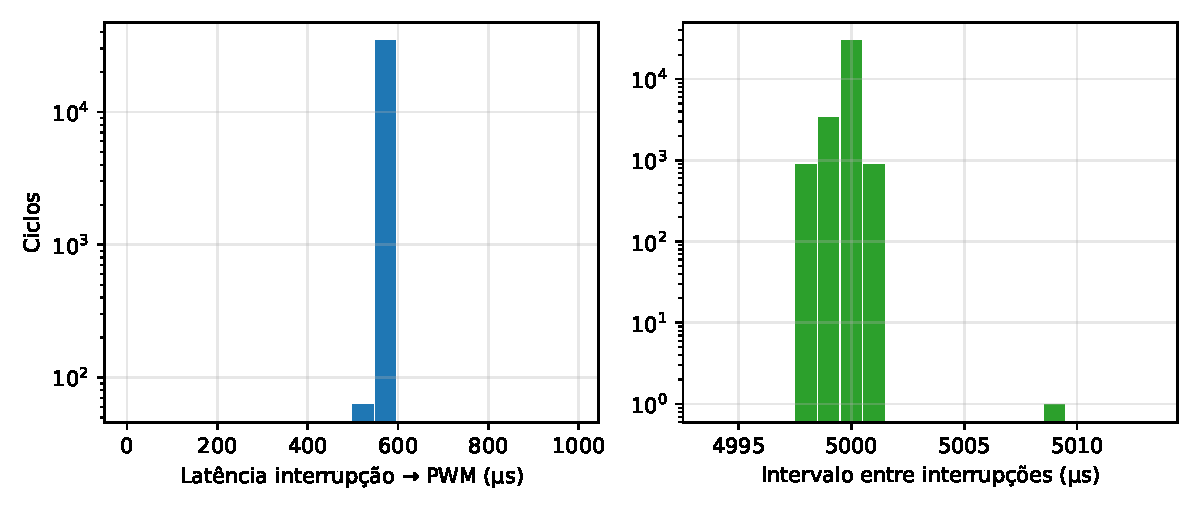
\includegraphics[width=.95\textwidth]{results/histogramas_tempo.pdf}
\fonte{Elaborado pelos autores (2026), dados da bancada.}
\end{figure}
O atraso total entre a interrupção e o PWM ficou em no máximo 580~$\mu$s, ou 11,6\% do prazo, dentro da faixa estimada (no limite inferior dela). A medida é dominada pela leitura I\textsuperscript{2}C de 14~bytes, feita por espera ativa, que ocupa cerca de 0,5~ms. O intervalo entre interrupções ficou entre 4\,998 e 5\,002~$\mu$s em todos os ciclos menos um, que chegou a 5\,009,5~$\mu$s: um \textit{jitter} de no máximo 11,2~$\mu$s, causado por outras interrupções curtas (SysTick, TIM4 da HAL, USART2). A tarefa levou no máximo 30,4~$\mu$s para acordar. A tarefa \texttt{control}, de maior prioridade, só pode ser atrasada por essas interrupções e por regiões críticas do núcleo; o \textit{mutex} \texttt{s\_dataMutex} é mantido apenas durante a cópia de uma estrutura de poucos bytes e conta com herança de prioridade. A transmissão pela UART, por espera ativa na tarefa \texttt{telem}, de prioridade menor, é interrompida pela tarefa \texttt{control}.

Há ainda o atraso dos dados, que independe do RTOS: o filtro digital do MPU6050 em 44~Hz atrasa o sinal em cerca de 5~ms \cite{mpu6050rm}, e como a amostragem do sensor (200~Hz) não é sincronizada com o TIM2, a amostra lida tem idade de 0 a 5~ms. Somados, esses efeitos têm a mesma ordem dos 9~ms de atraso puro identificados na planta (Tabela~\ref{tab:parametros}).

O maior valor observado é evidência experimental da bancada, mas não prova o pior caso de todas as execuções possíveis \cite{buttazzo2011}. A medição foi feita com a telemetria ativa; não foi repetida com ela desligada.

\chapter{DIFICULDADES ENCONTRADAS E SOLUÇÕES}\label{cap:dificuldades}

\section{AQUECIMENTO DO MOTOR E O INDUTOR}\label{sec:indutor}

O motor \textit{coreless} 0720 aquecia a ponto de não se poder tocá-lo. Os 12~V do driver sobre um motor de 3,7~V forçam um PWM de razão cíclica baixa, e esse motor tem indutância muito pequena (estimada em cerca de 7~$\mu$H, constante de tempo elétrica de poucos microssegundos, extrapolada de dados da maxon para motores \textit{coreless} de 8~mm \cite{maxonchoke}). O período de 10~$\mu$s do PWM a 100~kHz não alisa a corrente: ela acompanha cada pulso de 12~V, com picos de cerca de 2~A, e como o calor depende da corrente eficaz, e não da média, o motor dissipava cerca de 1,5~W contra 0,3~W em corrente contínua. Em 20~kHz e 1~kHz o modelo prevê corrente por pulso acima de 4~A, e o DRV8871 desarmava (religação em 3~ms), o que se ouvia como um zumbido agudo seguido do motor parando.

Duas observações apoiam essa explicação: o motor ligado direto em duas pilhas AA (cerca de 3~V, sem driver) não esquentou; e, em 200~kHz, a haste não equilibrou, provavelmente porque os pulsos ficam curtos demais para o driver, cujo pulso mínimo é de 800~ns \cite{drv8871ds}. Os valores de corrente vêm do cálculo em \texttt{firmware/tools/pwm\_heat.py}; a corrente de pico não foi medida.

A solução foi um indutor de potência em série com o motor. Antes, um capacitor em paralelo com o motor foi testado e não resolveu. O cálculo indicava 100~$\mu$H, e qualquer valor de 47 a 220~$\mu$H serve; foi instalado um de 220~$\mu$H e 3~A, com folga de corrente sobre os picos do motor. O driver, os 12~V e o PWM de 100~kHz em modo de freio continuaram iguais. Com o indutor, a corrente fica lisa: o consumo do motor ficou em torno de 0,4~A, em vez dos picos de cerca de 2~A previstos sem ele. O valor foi lido com multímetro pelo grupo; o ponto exato da medição não foi registrado.

\section{RUÍDO DO MPU6050 E FILTRAGEM}\label{sec:ruido}

Com o motor ligado, a leitura do ângulo pelo acelerômetro deixou de ser confiável. Nos registros: com a haste perto de $2^\circ$, o acelerômetro variou de $-58^\circ$ a $+18^\circ$; e em voo a mediana das amostras foi $+5^\circ$ (extremos de $-48^\circ$ a $+46^\circ$) enquanto a haste estava, de fato, perto de $+24^\circ$, como o giroscópio mostrou quando a haste caiu. Com o motor parado, acelerômetro e giroscópio concordavam. A vibração da hélice contamina a medida da gravidade; \citeonline{duong2025} mediram o mesmo efeito em um quadrirrotor com MPU6050.

A solução passou por camadas:
\begin{enumerate}[label=\alph*)]
 \item \textbf{Mecânica:} montagem do sensor com fita dupla face na haste e ligações soldadas, sem outro tratamento de vibração.
 \item \textbf{Filtro digital do sensor:} passa-baixas interno de 44~Hz e escalas de $\pm16$~g e $\pm1000^\circ$/s, para não saturar.
 \item \textbf{Filtro complementar com acelerômetro condicionado:} com o motor parado, constante de 2~s (um valor de 0,5~s, herdado do código Arduino, deixava o ruído passar). Em voo, a versão inicial usava só a integral do giroscópio, o que fez o erro crescer com o tempo (Seção~\ref{sec:deriva}); a versão atual corrige o ângulo pelo acelerômetro com constante de 30~s e descarta leituras que difiram da estimativa por mais de $25^\circ$. A calibração de 2~s continua exigindo a haste parada.
 \item \textbf{Filtro da derivada:} passa-baixas de 5~ms sobre a velocidade do giroscópio usada no termo D.
\end{enumerate}
Uma tentativa intermediária, que rejeitava amostras do acelerômetro cujo módulo saísse de 0,85 a 1,15~g, foi removida: não resolvia a polarização do ângulo.

\section{AJUSTE DO PID E O ANTI-\textit{WINDUP}}

Mesmo com ganhos ajustados, o PID não conseguia manter a haste estritamente na horizontal: com ganhos altos a haste oscilava (ciclo-limite) e com ganhos baixos subia devagar. A sequência foi: ganhos equivalentes aos do Arduino; ganhos de 1,0/0,5/0,15 (ciclo-limite entre $-10{,}8^\circ$ e $+5{,}4^\circ$); 0,30/0,15/0,09 (oscilação de $\pm3{,}7^\circ$, margem de fase de $3{,}6^\circ$); os ganhos de projeto, de margem de fase de cerca de $43^\circ$, e, depois do refino na bancada, $K_i=0{,}08$ com a mesma margem de fase de pior caso (Seção~\ref{sec:antiwindup} e Capítulo~\ref{cap:processo}). O integrador começa em 16\%, um pouco abaixo do PWM de pairar (cerca de 20\%); sem isso, com ganhos baixos, a haste levaria mais de 8~s para sair do repouso. O anti-\textit{windup} por integração condicional foi mantido porque, enquanto a saída está limitada entre 10\% e 32\%, um integrador livre acumula erro, e a simulação mostrou que isso pode multiplicar por dez o tempo de recuperação (Tabela~\ref{tab:windup}).

\section{DERIVA DO GIROSCÓPIO E A VOLTA COMPLETA DA HASTE}\label{sec:deriva}

Na primeira versão do filtro, com o motor ligado o ângulo era só a integral do giroscópio. Em 02/11/2026 isso apareceu na bancada de duas formas. Primeiro, a haste estabilizava visualmente cerca de $10^\circ$ acima da horizontal enquanto o firmware marcava $1{,}2^\circ$, com a placa ligada havia 12,8~min. Depois, com a haste segurada à mão no zero físico (nível de celular, velocidade nula e saída em 13,8\%), o acelerômetro marcou $-1{,}4^\circ$ (mediana; média $-1{,}9^\circ$, desvio $2{,}8^\circ$) e o firmware marcou $+11{,}6^\circ$, após 204~s ligado. A diferença de 13,5$^\circ$ em 190~s equivale a uns $4^\circ$/min, ou cerca de 0,07$^\circ$/s de viés residual do giroscópio, valor típico desse sensor. O controle seguia fielmente a estimativa errada: mantinha o firmware em $0{,}7^\circ$ e a haste se afastava do zero.

Em um dos ensaios a haste passou de $90^\circ$ e deu uma volta completa (o registro mostrou ângulos de $-180^\circ$ a $+180^\circ$). Acima de $90^\circ$ a gravidade deixa de puxar a haste para baixo e, com a marcha lenta de 10\%, ela passa por cima. Como a saída mínima nunca é zero, nada desligava o motor: faltava uma proteção por ângulo. Foram feitas duas mudanças: o corte por ângulo (Capítulo~\ref{cap:desenvolvimento}) e a correção lenta do ângulo pelo acelerômetro em voo, com constante de 30~s e janela de rejeição de $25^\circ$. A correção filtra o ruído de 8$^\circ$ do acelerômetro até cerca de $0{,}07^\circ$ na estimativa e mantém o ângulo atrelado à gravidade, ao custo de um erro fixo igual à polarização do acelerômetro em voo, que se compensa pelo \textit{setpoint}.

\section{DEMAIS PROBLEMAS}

\begin{itemize}
 \item \textbf{Mau contato na fiação do motor:} a haste ficou 8~s com saída máxima e só subiu quando o cabo foi mexido; os fios e as ligações foram soldados.
 \item \textbf{Ruído na recepção serial:} sem conversor ligado, o pino RX flutuante captava o ruído do motor; foi habilitado o \textit{pull-up} do PA3.
 \item \textbf{Queda do ST-Link:} a sonda ocasionalmente desconectava com o motor em funcionamento. Um ponto de atenção: interromper uma gravação deixa o TIM1 emitindo o último PWM sem controle, e o motor continua ligado.
\end{itemize}
